\documentclass[11pt,a4paper]{article}

\usepackage{kotex}
\usepackage{amsmath,amssymb,amsfonts,amsthm,bm}
\usepackage{graphicx}
\usepackage{pgfplots}
\pgfplotsset{compat=1.18}
% RdBu_r diverging colormap (ColorBrewer): blue=low (good) -> white -> red=high (bad),
% matching the v_ss contour colorscale used in the interactive HTML figures.
\pgfplotsset{
  colormap={RdBu_r}{
    rgb255=(5,48,97) rgb255=(33,102,172) rgb255=(67,147,195) rgb255=(146,197,222)
    rgb255=(209,229,240) rgb255=(247,247,247) rgb255=(253,219,199) rgb255=(244,165,130)
    rgb255=(214,96,77) rgb255=(178,24,43) rgb255=(103,0,31)
  }
}
\usetikzlibrary{arrows.meta, calc, positioning, decorations.pathreplacing, patterns, shapes.geometric}
% Styles/colors for the isometric flow-geometry figures (Fig.~1 and Fig.~2).
\definecolor{ohred}{HTML}{B23B2E}
\definecolor{rcblue}{HTML}{2F5FA6}
\tikzset{
  iso/.style={>=Latex, line join=round, line cap=round, scale=1.25,
    x={(0.87cm,-0.50cm)}, y={(-0.87cm,-0.50cm)}, z={(0cm,1.0cm)},
    every node/.style={font=\small}},
  rface/.style={fill=ohred!16, draw=ohred!72!black, line width=1pt},
  bface/.style={fill=rcblue!16, draw=rcblue!72!black, line width=1pt},
  nrm/.style={->, line width=1.2pt},
  flow/.style={->, line width=1pt, dash pattern=on 2.4pt off 2.4pt, gray!60!black},
}
\usepackage{booktabs}
\usepackage{algorithm}
\usepackage{algpseudocode}
\usepackage{float}
\usepackage{hyperref}
\usepackage{geometry}
\geometry{margin=25mm}

\title{Fast Candidate Generation for Support-Minimizing Build Orientation in 3D Printing Using a Support Flow Tensor Flow}
\author{InHwan Sul}
\date{}

\newtheorem{definition}{Definition}
\newtheorem{theorem}{Theorem}
\newtheorem{proposition}{Proposition}

\begin{document}

\maketitle

\begin{abstract}
Build orientation strongly affects support volume, material use, printing time, and post-processing quality in additive manufacturing.
Accurate support-volume evaluators, including the authors' previous GPU-based modified support-structure tomography (GPU-MSST; here denoted TOMO\_INT3),
can search a yaw--pitch grid, but they still evaluate every sampled direction and therefore retain a large fixed search cost.
This paper proposes a fast candidate generator, the Support Flow Tensor Field (SFTF), whose role is not to replace an accurate slicer or TOMO evaluator,
but to provide a small set of promising build-orientation candidates for subsequent local verification.

For each sampled build direction, SFTF estimates support tendency from two geometric cues: whether an overhang face can be supported by another visible face beneath it, and how much support must extend directly to the build plate.
The first cue is obtained by ray-cast face-to-face visibility and is accumulated as an asymmetric support-flow tensor; the second is a build-plate penalty.
The build-plate term can also be written as the Rayleigh contribution of a virtual ground receiver added to the tensor, so the main support cue remains within one augmented tensor formulation.
The derivation is given in the Appendix, while the main text emphasizes the resulting workflow: coarse spherical sampling, local resampling around good candidates, angular non-maximum suppression to report separated orientation basins, and final verification with TOMO or a slicer.

On stored TOMO\_INT3 grids, cross-validated SFTF candidates achieved a best-of-three support-volume ratio of $2.37$, compared with $3.63$ for PCA axes and $4.30$ for symmetric Support Tensor eigenvectors.
On a controlled five-group shape set ranging from primitives to meshes with about $10^6$ faces, Python SFTF reduced computation time by $1.4$--$34\times$ relative to a $3^\circ$ TOMO\_INT3 exhaustive sweep, and the C++ implementation by $10$--$5{,}160\times$.
The experiments also show that changing the exhaustive-sweep backend from INT3 to CUDA is not always faster on real and large meshes, whereas reducing the number of directions is consistently beneficial.
The method is therefore best interpreted as a fast, interpretable warm-start for support-minimizing build-orientation search.
\end{abstract}

\noindent\textbf{Keywords:} additive manufacturing, build orientation optimization, support minimization, candidate generation, support-flow tensor field, 3D printing

\section{Introduction}

\subsection{Build Orientation and the Support Structure Problem}

In additive manufacturing, and especially in the most widely used FDM (fused deposition modeling) method,
molten filament is stacked layer by layer~\cite{gibson}.
To print a downward overhang steeper than the critical angle (critical angle, $\theta_c$),
a support structure (support structure, SS) is needed to hold it up from below.
The support structure is a sacrificial structure that is removed after printing, but it consumes additional filament and print time,
and degrades surface quality through removal marks and staircasing.
Therefore the support volume is a key factor governing the cost and quality of FDM printing.

The scope of this paper is the standard single-build-direction setting in which support demand is mainly determined by downward overhangs and a printable critical angle.
This setting covers common slicer-style support estimation for extrusion-based 3D printing and also provides a geometric benchmark for support-volume evaluators such as MSST/TOMO.
It does not attempt to model process-specific thermal distortion, residual stress, or multi-axis deposition; these effects can be added later as additional objectives after promising orientation candidates have been generated.

Even for the same shape, the distribution of overhangs changes depending on the pose in which it is placed on the build plate,
so the build orientation directly affects the following factors.

\begin{itemize}
\item Support volume
\item Print time
\item Material usage
\item Surface quality
\item Print stability
\end{itemize}

Among these, finding the build orientation that minimizes the support volume is the optimal-orientation search problem that this study addresses.

\subsection{Related Work}
\label{sec:related}

Build orientation optimization and support structure reduction are long-studied topics in additive manufacturing design,
and prior approaches can be broadly divided into (i) \emph{orientation optimization}, which finds a build orientation with a small support volume,
(ii) \emph{support structure design}, which optimizes the shape of the support structure for a given orientation,
and (iii) \emph{design-stage approaches}, which reduce the support requirement itself by changing the geometry or topology of the part.

In orientation optimization, Das et al.\ voxelized the mesh and selected a build orientation that jointly considers the support volume and part error~\cite{das2017},
and Wang et al.\ used a layered depth--normal image representation and GPU acceleration to quickly process the geometric operations of complex polyhedra,
laying the foundation for voxel-based additive manufacturing computation~\cite{wang2010}.
Such explicit, voxel-based evaluation gives the support volume of a single direction accurately,
but when searching over directions exhaustively it incurs a large fixed cost independent of shape complexity
(shown quantitatively in \S\ref{sec:fivegroup}).

On the support structure design side, research that minimizes support volume with lattice or cellular structures is active.
Vaissier et al.\ pruned lattice support structures with a genetic algorithm to reduce material consumption~\cite{vaissier2019},
and Jiang et al.\ experimentally identified the printable critical overhang angle in extrusion-based additive manufacturing
to reduce unnecessary support~\cite{jiang2018}.
As attempts to reduce the support requirement at the design stage, Mirzendehdel and Suresh proposed topology optimization
that includes support structures as a constraint~\cite{mirzendehdel2016}, and Langelaar presented a unified formulation that simultaneously optimizes
part topology, support placement, and build orientation~\cite{langelaar2018}.
Meanwhile, Dai et al.\ demonstrated an alternative paradigm that achieves support-free printing using multi-axis motion~\cite{dai2018}.

In particular, a line of work that expresses the directional dependence of overhang directly as \emph{anisotropy} or a tensor
has developed within the topology-optimization community, and this is the family most closely related to the tensor formulation of the present study.
Gaynor et al.\ introduced a maximum overhang constraint into SIMP topology optimization, forcing each layer to be supported by the solid below it
within the self-supporting angle~\cite{gaynor2014}.
Garcke et al.\ penalized overhanging boundaries through anisotropic interface energy (an anisotropic interface energy of Wulff-shape type)
in a phase-field topology optimization, so that self-supportable boundary-normal directions are preferred~\cite{garcke2023}.
Shin et al.\ targeted multi-axis additive manufacturing and simultaneously optimized a deposition-direction-dependent material stiffness anisotropy tensor
$\mathbf{D}(\phi)=\mathbf{T}(\phi)\,\mathbf{D}_0\,\mathbf{T}(\phi)^T$, an overhang penalty, and the stage-wise build orientations~\cite{shin2025}.
On the industrial side, Smith and Hollenbeck patented a method that selects the build orientation of complex metal parts
with many orthogonal and internal faces---where support is hard to remove---so as to minimize support structure and surface distortion~\cite{smith2025patent}.

This study also shares with the anisotropy family above the idea of capturing the directionality of overhang with a tensor, but its position is complementary.
The tensors in those works represent the \emph{physical} anisotropy of material stiffness (Shin) or interface energy (Garcke)
\emph{inside} a PDE-constrained design optimization that changes the part topology/density,
with the build direction either fixed (Gaynor, Garcke) or co-optimized as a design variable (Shin).
By contrast, the Support Flow Tensor Field of this study is a purely geometric support-flow descriptor evaluated per candidate direction on a \emph{fixed} part,
used to \emph{rank} build orientations at low cost without redesigning the part.
That is, without changing the shape of the support structure or the part topology, and assuming standard FDM single-direction printing,
it focuses on the \emph{build orientation}, but rather than replacing the expensive exhaustive evaluation, it aims for a candidate generator and warm-start
that, in front of it, narrows down promising directions at low cost and passes them to an accurate verifier or the local verification of a commercial slicer.
The patent of Smith and Hollenbeck~\cite{smith2025patent} is close to this study in goal (selecting the build orientation of a fixed shape)
but is an industrial method whose procedure is not disclosed, whereas this study provides a transparent tensor cost and a verifier warm-start.
The next section first summarizes the implicit-estimation family that this study directly extends (shadow-volume-based MSST).

\subsection{Optimal Orientation Search: Explicit/Implicit Methods and MSST}

The optimal build orientation can be obtained explicitly or implicitly.
Explicit methods actually slice each candidate direction to generate G-code and directly compute the support volume.
They are accurate but expensive, so prior works, even after voxelizing the mesh and accelerating G-code generation with GPUs,
generally remained at single-direction evaluation due to the computational burden and could not be applied to exhaustive optimal-orientation search.

Implicit methods indirectly estimate the support volume without complex G-code generation.
Representatively, Ezair et al.\ observed that the volume of the support structure is similar to the shadow volume produced by a virtual sun~\cite{ezair}.
This is intuitive but holds only when the critical angle is $0^\circ$, i.e., when every overhang requires support.
The authors' prior work~\cite{msst} generalized this idea to an arbitrary critical angle
and developed it into ``modified support structure tomography (MSST).''%
\footnote{The authors' prior MSST~\cite{msst} and GPU-accelerated (GPU-MSST)~\cite{gpumsst} work. Public source code:
\url{https://github.com/cfms-lab/Tomo_GPU2024}.}

MSST divides the virtual ray into many rays and treats each ray's intersection with the surface as a ``pixel.''
Within a ``pixel slot'' that sorts pixels at the same $(x,y)$ location by their $Z$ coordinate,
it classifies upward-facing faces ($\alpha$) and downward-facing faces ($\beta$),
and estimates the support volume ($V_{ss}$) by subtracting the object volume ($V_o$) and the
non-overhang volume ($V_{nv}$) from the top-cover volume ($V_{tc}$) in the form $V_{ss}=V_{tc}-V_o-V_{nv}$.
This approach reproduced almost the same support volume as a commercial slicer on several standard meshes such as the Stanford Bunny.

\subsection{GPU-MSST and Remaining Limitations}

The only weakness of MSST was speed.
A single-direction computation of the $65$k-triangle Bunny takes about $1$ second,
and sweeping yaw--pitch at $1^\circ$ intervals requires $360\times360=129{,}600$ single-direction computations,
so a single optimal-orientation search takes $1$--$2$ minutes on a CPU.
The authors recently proposed GPU-MSST, which reconstructs MSST with GPU-friendly data structures (slot-based pixel data structure, triangle-split voxelization)~\cite{gpumsst},
shortening the same exhaustive search to about $10$ seconds and reporting on average $11.2\times$ acceleration relative to a high-end CPU and up to $62\times$ relative to a low-cost CPU.
In this paper we use this GPU-based MSST implementation as an accurate support-volume verifier and refer to it as TOMO\_INT3.

However, GPU-MSST also essentially searches the entire yaw--pitch grid \emph{exhaustively}.
That is, the acceleration made single-direction evaluation fast; it did not reduce the number of directions to be evaluated ($129{,}600$).
As a result, the search cost has a large fixed cost almost independent of shape complexity
(in \S\ref{sec:fivegroup} of the main text, even a cube with only $12$ faces takes about $4$ seconds for a $3^\circ$ TOMO\_INT3 sweep),
and is excessive for simple shapes or fast preliminary review.
Indeed, the prior work itself started from the observation that ``only a limited portion between the $\alpha$ faces and $\beta$ faces contributes to the final support structure,''
and presented, as future work, a tensorial approach (tentatively named shadow tensor) that reduces the evaluation targets.
This study is precisely the follow-up work in that direction.

\subsection{This Study: Support Flow Tensor Field}

The goal of this study is not to \emph{replace} the expensive exhaustive search, but to build a candidate generator
that quickly suggests promising build orientations in front of it, serving simultaneously as a slicer/TOMO warm-start.
By evaluating a low-cost support cost for each candidate direction on the sphere, it narrows down only a small number of promising orientations,
and feeds these into the local verification of TOMO\_INT3 or a commercial slicer, thereby reducing the overall search cost.

For this, a tensor that summarizes the shape is needed.
The simplest candidate is the symmetric tensor that collects the distribution of face normals with area weighting,
$M=\sum_i A_i m_i m_i^T$, which in this paper we call the ``Support Tensor'' as a comparison baseline.
However, as shown in \S\ref{sec:support-tensor-limit}, this symmetric tensor only captures the \emph{distribution} of normals
and cannot explain where the support structure actually flows from and to.
In particular, it does not reflect reentrant or internally occluded regions, the height to the build plate,
or the visibility changes that depend on the build orientation.

Therefore, for direction $n\in S^2$ this study directly evaluates an \emph{asymmetric} Support Flow Tensor Field $F(n)$
(\S\ref{sec:sftf}).
$F(n)$ accumulates, via ray casting, the face-to-face support ``flow'' from an overhang face toward the actual receiver face beneath it,
and is treated not as a simple eigenvector problem but as a per-direction cost evaluation problem.
Also, as the core unifying perspective of this study, the build-plate support cost is formulated not as a separate scalar penalty but as
the Rayleigh contribution obtained when adding a ``virtual ground node whose normal is the build direction'' to the flow tensor.
In this way, face-to-face self-support and build-plate support are unified into a single flow tensor
(unified Rayleigh cost $\tilde R=R+B$, \S\ref{sec:groundnode}),
and in the quantitative analysis (\S\ref{sec:unified}) we confirm that this unified term drives the predictive power.

In summary, the contributions of this study are as follows.
\begin{itemize}
\item We formulate build-orientation selection as a fast candidate-generation problem before accurate TOMO/slicer verification, rather than as a complete replacement for exhaustive support-volume search.
\item We define an asymmetric Support Flow Tensor Field $F(n)$ for each build orientation, using ray casting to distinguish internal face-to-face self-support from support that must reach the build plate.
\item We show that the build-plate support cost can be interpreted as the Rayleigh contribution of a virtual ground receiver added to the flow tensor (Eq.~\eqref{eq:Rtilde}); the derivation is kept in the Appendix so that the main text can focus on the AM workflow.
\item Through correlation analysis, ablation, and cross-validation on a stored TOMO\_INT3 grid, we identify which terms actually predict support volume and verify the advantage over PCA and symmetric Support Tensor eigenvector baselines.
\item On a difficulty-controlled five-group shape set, including meshes with about $10^6$ faces, we compare Python SFTF and C++ SFTF with TOMO\_INT3/TOMO\_CUDA $3^\circ$ exhaustive sweeps and show that reducing the number of evaluated orientations gives a larger and more stable speed gain than changing the exhaustive-sweep backend alone.
\end{itemize}

For readability, the main text can be read as a four-step workflow:
(1) detect direction-dependent overhangs,
(2) estimate whether they can flow to another face or must reach the build plate,
(3) rank a small candidate pool of build orientations, and
(4) verify only those candidates with TOMO or a slicer.
The algebraic proof that the build-plate term can be absorbed into an augmented tensor is provided in Appendix~\ref{sec:appendix-proof}.

\section{The Baseline (Symmetric) Support Tensor and Its Limitations}
\label{sec:support-tensor-limit}

\paragraph{Terminology (important).}
Since two tensors with similar names appear in this paper, we first distinguish them.
The \emph{Support Tensor} is a \textbf{symmetric} tensor that collects the distribution of face normals with area weighting;
it is \emph{not} newly proposed by this study but is a classical construction used as a comparison baseline.
It belongs to the same family as the orientation tensor (or fabric tensor) of fiber/particle mechanics
or the structure tensor of image processing, i.e., the ``second moment of the normal vectors.''%
\footnote{The symmetric tensor $\sum_i A_i m_i m_i^T$ is the (area-weighted) outer-product sum of the normals $m_i$, a classical shape descriptor of the structure
tensor / orientation tensor family. See: \cite{kanatani1984}.}
By contrast, what this study newly proposes is the direction-dependent \textbf{asymmetric}
tensor of the next section (\S\ref{sec:sftf}), the \emph{Support Flow Tensor Field} $F(n)$.
In short, the ``Support Tensor'' is an existing baseline, and the ``Support Flow Tensor Field'' is the contribution of this study.
Meanwhile, the anisotropic interface-energy or stiffness tensors used to handle overhang in topology optimization~\cite{garcke2023,shin2025}
form yet a third category distinct from both: they are not descriptors of the directional cost of a fixed shape
but \emph{physical} anisotropy models within a design optimization that redesigns the part (\S\ref{sec:related}).

\paragraph{Definition and Properties.}
The baseline (symmetric) Support Tensor is defined as
\begin{equation}
M
=
\sum_i
A_i m_i m_i^T
\end{equation}
Here $A_i$ is the area of triangular face $i$, and $m_i$ is its outward normal.
Since $M$ is a symmetric positive semidefinite matrix,%
\footnote{A symmetric matrix such that $x^TMx\ge0$ for all vectors $x$. This means all eigenvalues are $\ge0$.
See: \cite{hornjohnson}}
an eigenvector%
\footnote{A direction $x$ satisfying $Mx=\lambda x$, representing the axes that the matrix ``stretches'' most strongly.
See: \cite{golubvanloan}}
interpretation is possible.
That is, the eigenvectors of $M$ tell us which direction the shape's normals point on average (the principal direction).

\paragraph{Limitations.}
However, $M$ only captures the \emph{distribution} of normals and not the \emph{process} by which the support structure is actually generated.
Specifically, $M$ does not include the following information.

\begin{itemize}
\item Which faces are overhangs in a particular direction
\item Whether there is another actually supportable face beneath an overhang face
\item The height or distance to the support target
\item The region that the build plate must directly support
\item The asymmetric face-to-face support flow
\end{itemize}

Therefore, the eigenvectors of the Support Tensor can explain the statistical directionality of the shape,
but they do not always coincide with the optimal direction of the support volume that the slicer computes.
This limitation is the starting point for introducing a per-direction asymmetric flow tensor in the next section.

\section{Per-Direction Support Flow Tensor Field}
\label{sec:sftf}

We take the build orientation as a unit vector
\begin{equation}
n\in S^2, \qquad \|n\|=1
\end{equation}
Letting the centroid of face $i$ be $c_i$, the outward normal $m_i$, and the area $A_i$,
the overhang coefficient at direction $n$ is defined as
\begin{equation}
O_i(n)=\max(0,-m_i\cdot n)
\end{equation}

Let $j$ be the first valid face encountered by casting a ray in direction $-n$ from overhang face $i$.
The height difference is then
\begin{equation}
h_{ij}(n)=(c_i-c_j)\cdot n
\end{equation}
and only the case $h_{ij}>0$ is recognized as a support flow.

The face-to-face influence is set as
\begin{equation}
w_{ij}(n)
=
\frac{O_i(n)}{1+\alpha h_{ij}(n)}
\end{equation}
The current implementation uses
\begin{equation}
\alpha = \frac{1}{D}
\end{equation}
where $D$ is the bounding box diagonal of the input mesh.

Therefore the Support Flow Tensor for direction $n$ is computed as
\begin{equation}
F(n)
=
\sum_{(i,j)\in \mathcal{R}(n)}
w_{ij}(n)
A_iA_j
m_i m_j^T
\end{equation}
Here $\mathcal{R}(n)$ is the set of valid face-to-face support relationships obtained by ray casting.%
\footnote{A technique that shoots a ray to find the first surface it encounters. Here it is used to shoot a ray
from an overhang face in the direction opposite the build direction ($-n$) to find the receiver face below.
See: \cite{roth1982}}
Since $F(n)$ is a sum of $m_i m_j^T$, it is in general not a symmetric matrix.

\section{Ray Casting and Valid Support Relationships}

For each candidate direction $n$, ray casting every overhang face would be computationally expensive.
Therefore, the current implementation selects source faces by deterministic stratified sampling%
\footnote{Stratified sampling. A method that divides the whole into several intervals (strata) and then draws samples from each stratum,
obtaining a more evenly representative sample than simple random sampling (stratified sampling). See: \cite{cochran1977}}
in proportion to the overhang contribution
\begin{equation}
A_iO_i(n)
\end{equation}
The number of rays is set according to the number of faces $N_f$ as
\begin{equation}
K_{ray}
=
\mathrm{clip}(0.02N_f,500,3000)
\end{equation}

To avoid self-intersection, the ray origin is slightly shifted as
\begin{equation}
r_i(0)=c_i-\varepsilon n
\end{equation}
and the ray direction is $-n$.
The current implementation uses
\begin{equation}
\varepsilon = 10^{-6}D
\end{equation}

A valid receiver face $j$ must satisfy the following conditions.

\begin{enumerate}
\item $j\ne i$.
\item The ray distance is sufficiently positive.
\item $h_{ij}(n)>10^{-5}D$.
\item The receiver normal faces the build direction sufficiently.
\end{enumerate}

The last condition is implemented as
\begin{equation}
m_j\cdot n > \eta
\end{equation}
and currently uses $\eta=0.05$.
This condition removes vertical or flipped faces that are hard to regard as actual receiver faces even if the ray reached them.

\section{Build Plate Term}

An overhang face for which ray casting cannot find a support face below must eventually be held up by the build plate or by a separate support structure.
The current implementation computes this term as a scalar, but
as shown in \S\ref{sec:groundnode}, it is exactly equal to the Rayleigh contribution obtained when adding the build plate to the flow tensor as a virtual receiver.

The build-plate height reference for direction $n$ is defined as
\begin{equation}
z_{plate}(n)=\min_{v\in V} v\cdot n
\end{equation}
The height of face $i$ to the build plate is
\begin{equation}
h_{iP}(n)=c_i\cdot n-z_{plate}(n)
\end{equation}

Letting $\mathcal{B}(n)$ be the set of source faces with no valid face-to-face hit,
the build-plate support penalty is computed as
\begin{equation}
B(n)
=
\sum_{i\in\mathcal{B}(n)}
O_i(n)A_i\left(1+\alpha h_{iP}(n)\right)
\end{equation}
This term increases the cost the more a tall overhang directly requires support all the way to the build plate.

\subsection{Virtual Ground Node Interpretation of the Build Plate}
\label{sec:groundnode}

$B(n)$ looks like a scalar penalty added outside the tensor,
but it is in fact equivalent to the Rayleigh contribution obtained when adding the build plate as a virtual receiver (ground node)
to the face-to-face flow tensor $F(n)$.
The idea is that the support-face normal of the build plate is exactly the build direction $n$
($m\cdot n=1$, i.e., the limiting receiver that faces most upward),
so a face $i\in\mathcal{B}(n)$ supported by the plate can be treated as a ``flow pair with a virtual node whose normal is $n$.''
Adding these virtual pairs to the face-to-face flow tensor yields an \emph{augmented flow tensor} $\tilde F(n)$,
whose symmetric part $\tilde F_s(n)$ satisfies the exact identity
\begin{equation}
\tilde R(n)
=
\max\!\big(0,\,-n^T\tilde F_s(n)\,n\big)
=
R(n)+B(n)
\label{eq:Rtilde}
\end{equation}
That is, the unified Rayleigh cost $\tilde R$ equals the sum of the face-to-face Rayleigh term $R$ and the build-plate penalty $B$.
The explicit construction of $\tilde F(n)$ and the term-by-term derivation of Eq.~\eqref{eq:Rtilde} are given in Appendix~\ref{sec:appendix-proof}.
This equivalence was also numerically confirmed as $\max|\tilde R-(R+B)|<10^{-12}$ over the entire candidate pool of the five stored meshes
(about $1{,}292$ candidates each) (\S\ref{sec:unified}).

The significance of this reformulation is twofold.
First, the build-plate cost that accounts for most of the predictive power (\S\ref{sec:ablation})
turns out to be not an ad-hoc scalar but a term of the flow tensor, justifying the ``tensor'' formulation.
Second, the build plate is not a separate mechanism but is unified as
``the limit of face-to-face self-support (a fully horizontal receiver)''---
every overhang flows to a receiver, and that receiver is either another face or the build plate.
The asymmetry of the height convention is intentional.
The face-to-face weight uses attenuation $1/(1+\alpha h)$ (distant self-support is weakened),
while the plate term uses amplification $(1+\alpha h)$ (a tall support column is costly).
That this sign difference is not arbitrary is verified by quantitative comparison with other conventions in \S\ref{sec:unified}.

\begin{figure}[H]
\centering

\includegraphics[width=\textwidth]{pics/FTree4x_fig1_unified_flow.pdf}
\caption{Unified support-flow interpretation on the nonconvex FTree4x example. The semi-transparent mesh is rotated $180^\circ$ about the build direction $n$ for visibility. (a) Face-to-face flow: an overhang face $i$ casts a ray along $-n$ and is supported by a real receiver face $j$, contributing $m_im_j^T$ with support height $h_{ij}$. (b) Build-plate flow: when no valid receiver face exists below the overhang, the build plate is treated as a virtual receiver whose normal is $n$, contributing $m_in^T$ with support height $h_{iP}$.}
\label{fig:unified-flow}
\end{figure}

\section{Per-Direction Objective Function}

\begin{figure}[H]
\centering
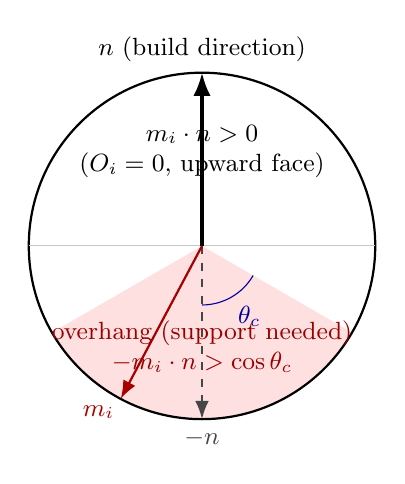
\begin{tikzpicture}[>=Latex, every node/.style={font=\small}]
  \def\R{2.2}
  % support-needed cone (overhang) around -n, half-angle theta_c
  \fill[red!12] (0,0) -- (-150:\R) arc[start angle=-150, end angle=-30, radius=\R] -- cycle;
  % unit circle of possible face-normal directions
  \draw[thick] (0,0) circle (\R);
  \draw[gray!45] (-\R,0) -- (\R,0);
  % build direction and its opposite
  \draw[->, very thick] (0,0) -- (0,\R) node[above] {$n$ (build direction)};
  \draw[->, thick, gray!55!black, dashed] (0,0) -- (0,-\R) node[below] {$-n$};
  % a sample overhang normal inside the cone
  \draw[->, thick, red!65!black] (0,0) -- (-118:\R) node[below left=-2pt] {$m_i$};
  % theta_c angle between -n and the cone edge
  \draw[blue!60!black] (-90:0.75) arc[start angle=-90, end angle=-30, radius=0.75];
  \node[blue!60!black] at (-56:1.08) {$\theta_c$};
  % region labels
  \node[align=center] at (0,1.2) {$m_i\cdot n>0$\\($O_i=0$, upward face)};
  \node[red!60!black, align=center] at (0,-1.28) {overhang (support needed)\\$-m_i\cdot n>\cos\theta_c$};
\end{tikzpicture}
\caption{Geometric meaning of the overhang coefficient $O_i(n)=\max(0,-m_i\cdot n)$. The possible face-normal directions
are shown on a unit circle with respect to the build direction $n$. The upper semicircle ($m_i\cdot n>0$) consists of upward faces with $O_i=0$,
and the lower shaded region is the cone of half-angle $\theta_c$ around $-n$, where faces with $-m_i\cdot n>\cos\theta_c$ are overhangs that actually
require support. $O_i$ grows the more the normal aligns with $-n$ (the further down it goes).}
\label{fig:overhang-coeff}
\end{figure}

To use the asymmetric tensor $F(n)$ as a directional cost, we define the symmetric component as
\begin{equation}
F_s(n)=\frac{F(n)+F(n)^T}{2}
\end{equation}

The initial approach used $n^TF_s(n)n$ directly, but experiments showed that under strong support flow the sign of the value could become negative,
flipping the alignment direction.
Therefore the current implementation converts the Rayleigh term%
\footnote{Rayleigh quotient: for a symmetric matrix $A$ and vector $x$, the scalar defined as $\dfrac{x^TAx}{x^Tx}$.
Since $\|n\|=1$ here, $n^TF_s(n)\,n$ itself is the Rayleigh quotient at direction $n$,
and we flip its sign to interpret it as a ``support cost.'' (A quantity closely related to eigenvalues; \cite{hornjohnson})}
into a non-negative support cost.

\begin{equation}
R(n)=\max\left(0,-n^TF_s(n)n\right)
\end{equation}

The face-to-face support volume term is set as
\begin{equation}
P(n)
=
\sum_{(i,j)\in\mathcal{R}(n)}
\left(
\frac{O_i(n)}{1+\alpha h_{ij}(n)}A_iA_j
\right)
\left(1+\alpha h_{ij}(n)\right)
\end{equation}
Here the height attenuation factor $1/(1+\alpha h_{ij})$ included in the face-to-face influence $w_{ij}$ and the outer $(1+\alpha h_{ij})$ cancel each other,
so $P(n)$ ultimately simplifies to
\begin{equation}
P(n)
=
\sum_{(i,j)\in\mathcal{R}(n)}
O_i(n)A_iA_j
\end{equation}
That is, $P(n)$ represents the area-weighted overhang amount itself over the valid hits,
and the height dependence is intentionally removed.
This is a choice to keep the height attenuation in the tensor $F(n)$ so as to weaken the contribution of distant face-to-face flows,
while interpreting the face-to-face support volume term $P(n)$ as the pure self-supportable area amount.

Using the augmented tensor of \S\ref{sec:groundnode}, the Rayleigh term $R$ and the build-plate term $B$
merge into a single unified Rayleigh cost $\tilde R=R+B$ (Eq.~\eqref{eq:Rtilde}).
Therefore the final objective function can be written as the sum of the unified tensor term and the face-to-face support volume
\begin{equation}
J(n)
=
\lambda_R R(n)
+
\lambda_P P(n)
+
\lambda_B B(n)
=
\underbrace{\tilde R(n)}_{R+B}
+
P(n)
\end{equation}
with ($\lambda_R=\lambda_P=\lambda_B=1$),
and from the unified-tensor perspective it is interpreted as ``the Rayleigh support cost $\tilde R$ of the augmented flow tensor
plus the face-to-face support area amount $P$.''
As shown in \S\ref{sec:unified}, $\tilde R$ itself is a better predictor than $J$,
because the summed $P$ acts as a negative signal.
In the initial implementation, from the singular values%
\footnote{Singular value and singular value decomposition (SVD): the non-negative scale factors that appear when decomposing an arbitrary matrix into rotation--scale--rotation,
representing how much the matrix ``stretches'' along each axis.
For the non-symmetric $F(n)$, singular values are used instead of eigenvalues. See: \cite{golubvanloan}}
$\sigma_1\ge\sigma_2\ge\sigma_3\ge0$ of $F(n)$
we added a nuclear score%
\footnote{Nuclear norm: the sum of singular values $\sum_k\sigma_k$. A type of Schatten norm,
a measure of the overall ``size'' of a matrix (a type of matrix norm). See: \cite{hornjohnson}}
$S(n)=\sum_k\sigma_k(n)$ and a $\sigma_1(n)$ term with weight $0.05$, but
in the ablation of \S\ref{sec:ablation} these two terms were confirmed not to change the candidate selection at all, so they were excluded from the objective function.
The singular values are kept only as auxiliary features for post-processing rank tuning.%
\footnote{In this paper, ``rank tuning'' is not a standard term but refers to the post-processing procedure of this study.
Each feature is normalized to its rank within the candidate set ($0$\,$\sim$\,$1$) (see the formula in \S\ref{sec:cv}),
and then linear weights are learned on these rank-normalized features to re-rank the candidates.
For the concepts of rank and rank correlation, see \cite{spearman1904}.}
(\S\ref{sec:cv}).
The optimal build orientation is defined as
\begin{equation}
n^* = \arg\min_{n\in S^2} J(n)
\end{equation}

\section{Spherical Sampling and Local Re-search}

Using only three eigenvectors does not sufficiently reflect the asymmetry and direction dependence of the Support Flow Tensor Field.
Therefore the current implementation uses the following two-stage search that follows a simple coarse-to-fine strategy
of evaluating a sparse global sample and then densely resampling only around promising candidates.

\begin{enumerate}
\item Generate $512$ coarse directions by the Fibonacci sphere~\cite{saff1997,gonzalez2010} method.%
\footnote{A method that scatters points nearly uniformly on a sphere using the golden angle ($\approx137.5^\circ$),
commonly used to obtain evenly distributed direction samples (the $137.508^\circ$ rotation in the code is this).
For classical results on quasi-uniform distributions of points on a sphere, see Saff and Kuijlaars~\cite{saff1997};
for the spherical application of the Fibonacci lattice and its uniformity analysis, see González~\cite{gonzalez2010}.}
\item Compute $J(n)$ for each direction.
\item Select the top $12$ candidates, but remove directions that are too close to each other.
\item Resample around each top candidate with $2^\circ$, $4^\circ$, $6^\circ$, $8^\circ$ cones.
\item For each cone angle, evaluate $16$ azimuths.
\item Combine the coarse and refined candidates and re-sort.
\item Finally return the top 3 directions that are at least $3^\circ$ apart from each other.
\end{enumerate}

This approach is faster than densely evaluating the entire sphere,
while still being able to reflect sensitivity to small angular changes around the optimal direction.

\begin{figure}[H]
\centering
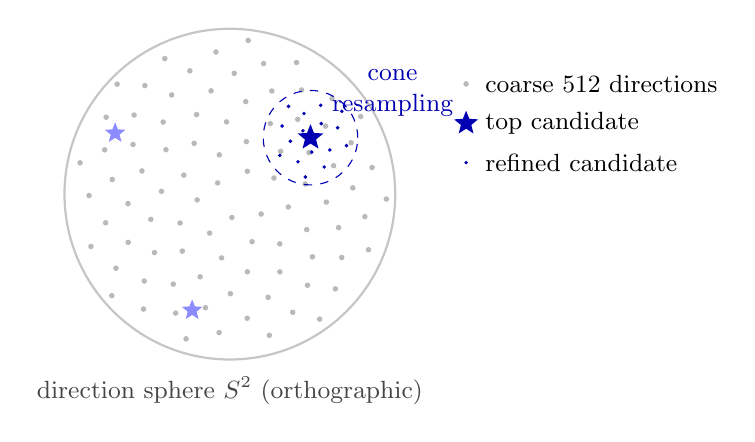
\begin{tikzpicture}[>=Latex, every node/.style={font=\small}]
  % direction sphere (orthographic disk)
  \draw[thick, gray!45] (0,0) circle (2.1);
  \node[gray!55!black] at (0,-2.5) {direction sphere $S^2$ (orthographic)};
  % coarse Fibonacci-like samples
  \foreach \k in {1,...,90}{
    \pgfmathsetmacro{\rad}{2.0*sqrt(\k/90)}
    \pgfmathsetmacro{\ang}{\k*137.508}
    \fill[gray!55] (\ang:\rad) circle (1.0pt);
  }
  % top candidates (stars)
  \node[star, star points=5, star point ratio=2.3, fill=blue!70!black, inner sep=1.5pt] at (35:1.25) {};
  \node[star, star points=5, star point ratio=2.3, fill=blue!45, inner sep=1.2pt] at (-108:1.55) {};
  \node[star, star points=5, star point ratio=2.3, fill=blue!45, inner sep=1.2pt] at (152:1.65) {};
  % cone refinement around the best candidate
  \draw[dashed, blue!70!black] (35:1.25) circle (0.6);
  \foreach \j in {1,...,16}{
    \pgfmathsetmacro{\rr}{0.52*sqrt(\j/16)}
    \pgfmathsetmacro{\aa}{\j*137.508}
    \fill[blue!70!black] ($(35:1.25)+(\aa:\rr)$) circle (0.7pt);
  }
  \node[blue!70!black, align=center, above right=6pt] at (35:1.25) {cone\\resampling};
  % legend
  \fill[gray!55] (3.0,1.4) circle (1.0pt); \node[right] at (3.12,1.4) {coarse 512 directions};
  \node[star, star points=5, star point ratio=2.3, fill=blue!70!black, inner sep=1.4pt] at (3.0,0.9) {};
  \node[right] at (3.12,0.9) {top candidate};
  \fill[blue!70!black] (3.0,0.4) circle (0.7pt); \node[right] at (3.12,0.4) {refined candidate};
\end{tikzpicture}
\caption{Two-stage direction search. After evaluating coarse candidates (gray, $512$) that sparsely cover the sphere via the Fibonacci sphere,
the regions around the top candidates (stars) are densely resampled with $2^\circ$--$8^\circ$ cones (blue dots)
to reflect sensitivity near the optimal direction. Local precision is obtained without densely evaluating the entire sphere.}
\label{fig:spherical-sampling}
\end{figure}

\section{Computational Acceleration and Final Candidate Rescoring}

Since the per-direction Support Flow Tensor Field casts many rays for each candidate direction,
a direct implementation has its computational bottleneck mostly in ray--triangle intersection~\cite{moller1997}.
The initial implementation obtained all hits for each ray and then
sorted by distance to find the first valid receiver face.
However, since for most rays the nearest hit is immediately the valid hit,
computing all hits every time creates unnecessary cost.

The current implementation first performs a first-hit query with
\begin{equation}
\mathrm{multiple\_hits}=\mathrm{False}
\end{equation}
Only when this first hit violates the self-face, too-short distance, negative height difference, or receiver normal condition
is the existing multiple-hit query performed as a fallback for that ray.
That is, over the entire ray set $\mathcal{Q}$, only
\begin{equation}
\mathcal{Q}_{fallback}
=
\{q\in\mathcal{Q}\mid \mathrm{firstHit}(q)\ \mathrm{is\ invalid}\}
\end{equation}
is searched additionally.
This strategy maintains the existing exact valid-hit selection rule, while
reducing the number of intersection candidates and the sorting cost for most rays.

Also, the face normals, areas, centroids, vertex arrays,
bounding box diagonal $D$, $\alpha=1/D$, ray offset $\varepsilon$, and height tolerance, which used to be recomputed for each candidate direction,
were computed only once per mesh and cached.
For this, the current implementation shares
\begin{equation}
\mathcal{D}_{mesh}
=
\{m_i,A_i,c_i,V,D,\alpha,\varepsilon,\varepsilon_h\}
\end{equation}
across the entire Support Flow evaluation.

In profiling on the Bunny 1k mesh,
the existing direction evaluation time was about $15.7$ seconds, but
after applying first-hit fallback and mesh surface data caching it decreased to about $1.5$ seconds.
On the same mesh, the selected top direction, score, and hit count matched those of the existing multiple-hit method.
Therefore this optimization can be viewed as an implementation-level acceleration that reduces only the computational amount without changing the meaning of the algorithm.

\subsection{Final Candidate Rescoring Based on TOMO Results}

The original objective function $J(n)$ was effective for candidate generation and local re-search, but
it was not always well aligned with the actual support volume $v_{ss}$ of TOMO\_INT3 when choosing the final top 3 candidates.
In particular, a direction with a small $B(n)$ term is not always a direction with a small actual support volume,
and a candidate with too small a face-to-face flow amount and hit count may not actually form sufficient self-support relationships.

Therefore, after the coarse and refined candidate pool has been generated, the current implementation applies a final rank-based rescoring step.
The rescoring uses the intra-pool ranks of $J$, $R$, $P$, $B$, hit count, and singular-value descriptors, rather than their raw numerical values.
This keeps the candidate generator itself simple and geometric, while allowing the final ordering to incorporate empirical feedback from TOMO or a slicer.
The detailed formula and the calibration weights used for the reported in-sample values are given in Appendix~\ref{sec:appendix-ranktuning}.

Two points are important for interpreting the results.
First, the calibrated weights are not claimed to be universal physical constants; they are an example of using accurate support-volume feedback to rank an already small candidate pool.
Second, the paper reports Leave-One-Mesh-Out cross-validation in \S\ref{sec:cv}, so the reader can distinguish the optimistic in-sample ranking from a more conservative generalization estimate.

\section{Algorithm Overview}

\begin{algorithm}[H]
\caption{Augmented (ground-node) Support Flow Tensor Evaluation with Final Rank Tuning}
\begin{algorithmic}[1]
\For{each sampled build direction $n$}
    \State Normalize $n$
    \State Compute $O_i(n)=\max(0,-m_i\cdot n)$ for all faces
    \State Select $K_{ray}$ source faces by stratified sampling with weight $A_iO_i(n)$
    \State Initialize $\tilde F\gets 0$ \Comment{augmented flow tensor (face-to-face + virtual ground node)}, $P\gets 0$
    \For{each sampled source face $i$}
        \State Cast ray from $c_i-\varepsilon n$ along $-n$
        \State Find the first valid receiver face $j$
        \If{valid $j$ exists}
            \State $h_{ij}\gets(c_i-c_j)\cdot n$;\quad $w_{ij}\gets O_i(n)/(1+\alpha h_{ij})$
            \State $\tilde F\gets \tilde F+w_{ij}A_iA_jm_im_j^T$ \Comment{face-to-face flow}
            \State $P\gets P+w_{ij}A_iA_j(1+\alpha h_{ij})$
        \Else
            \State $h_{iP}\gets c_i\cdot n-z_{plate}(n)$
            \State $\tilde F\gets \tilde F+A_i(1+\alpha h_{iP})\,m_in^T$ \Comment{build-plate flow (virtual ground node)}
        \EndIf
    \EndFor
    \State $\tilde F_s\gets(\tilde F+\tilde F^T)/2$
    \State $\tilde R\gets\max(0,-n^T\tilde F_sn)$ \Comment{$=R+B$, Eq.~\eqref{eq:Rtilde}}
    \State $J(n)\gets \tilde R+P$
    \State (singular values $\sigma_1,\sigma_2,\sigma_3$ are computed from the face-to-face subtensor $F$ only as auxiliary features for rank tuning)
\EndFor
\State Generate refined directions around the best coarse candidates under $J(n)$
\State Evaluate $J(n)$ and feature vector $x(n)$ for all coarse and refined candidates
\State Rank-normalize each feature inside the candidate set
\State Compute final tuning score $T(n)$
\State Return directions sorted by $T(n)$ with angular non-maximum suppression
\end{algorithmic}
\end{algorithm}

In the implementation, instead of accumulating the build-plate term into the tensor, it is summed separately as a scalar $B$
to equivalently compute $\tilde R=R+B$ (the equivalence of \S\ref{sec:groundnode}, numerically confirmed within $10^{-12}$).
The above pseudocode makes explicit the unified-tensor form that is mathematically the same as that scalar accumulation.
The face-to-face subtensor $F$ is the part of $\tilde F$ excluding the ground-node term, and is used only for computing the singular value features.

\section{Comparison Targets and Evaluation Protocol}
\label{sec:protocol}

We first define the comparison targets and evaluation procedure used in the quantitative analyses up to \S\ref{sec:fivegroup}.
The comparison targets are as follows.

\begin{enumerate}
\item PCA-based direction
\item Existing Support Tensor eigenvector direction
\item Initial tensor-eigenvector direction
\item This study's Support Flow Tensor Field direction
\item TOMO\_INT3 or commercial-slicer-based $v_{ss}$ optimal direction
\end{enumerate}

For each mesh, we generate a $v_{ss}$ contour at $1^\circ$ intervals under a critical angle of $60^\circ$,
and evaluate how close the $v_{ss}$ value at our method's top candidate directions is to the global optimum.
Even if the direction coordinates do not match exactly, if the $v_{ss}$ values are similar we regard them as optimal orientations of the same level.
Also, considering the case where the global optimum appears scattered across multiple basins,
we compare angularly separated top-$k$ basin representatives rather than simple top-$k$ grid points.
The candidate basins proposed by SFTF are re-input to TOMO\_INT3 as a single initial orientation with angle step $0^\circ$
to directly measure the Mss,
and based on that measured value we mark the measured optimal and measured worst basins.

\section{Comparison with Stored TOMO\_INT3 Results}

To verify the current implementation, we used the
\texttt{*\_tomo\_int3\_vss\_grid\_1deg\_60deg.npz} files provided with the validation data.
Each file contains the TOMO\_INT3 support volume $v_{ss}$ computed on a yaw--pitch $1^\circ$ grid,
and the global minimum direction of that grid.
In the comparison process, instead of recomputing the TOMO grid,
we mapped the top directions proposed by the current Support Flow Tensor Field onto the TOMO grid,
and read the $v_{ss}$ value at that location to compare with the global optimum.

The TOMO yaw--pitch corresponding to an SFTF direction $n$ was chosen as the grid point that best satisfies,
for TOMO's rotation matrix $R(yaw,pitch,0)$,
\begin{equation}
R(yaw,pitch,0)n \approx e_z
\end{equation}
Since a direction vector and its sign reversal can represent the same build axis,
both $n$ and $-n$ were evaluated and the smaller $v_{ss}$ value was used as the signed result.

\begin{table}[H]
\centering
\caption{Comparison of the stored TOMO\_INT3 $v_{ss}$ grid with the current SFTF candidates.
Ratio is the ratio of the SFTF candidate's $v_{ss}$ to the TOMO global optimal $v_{ss}$.}
\label{tab:sftf-tomo-comparison}
\begin{tabular}{lrrrrr}
\toprule
Mesh & TOMO best & SFTF score1 & Ratio & SFTF best-of-3 & Ratio\\
\midrule
Bunny 69k & 3201.39 & 4665.85 & 1.46 & 4665.85 & 1.46\\
manikin & 4657.72 & 8675.96 & 1.86 & 8675.96 & 1.86\\
dragon 100k & 24446.98 & 45804.41 & 1.87 & 39547.57 & 1.62\\
happy 50k & 2112.47 & 25467.94 & 12.06 & 23727.49 & 11.23\\
lucy 50k & 5036.14 & 14192.68 & 2.82 & 14192.68 & 2.82\\
\bottomrule
\end{tabular}
\end{table}

As Table~\ref{tab:sftf-tomo-comparison} shows,
SFTF with rank tuning applied selected candidates closer to the TOMO optimum than the existing raw score for Bunny, manikin, and dragon.
In particular, Bunny's signed score1 ratio improved from about $3.03$ to $1.46$,
manikin from about $3.99$ to $1.86$,
and dragon's best-of-3 signed ratio from about $2.01$ to $1.62$.
By contrast, the improvement was limited for happy and lucy.

However, the rank tuning results in Table~\ref{tab:sftf-tomo-comparison} are in-sample values measured on the very mesh set on which the weights were calibrated.
Therefore these numbers are not generalization performance but a fit to the calibration set,
and whether the weights are overfit and the performance on unseen meshes are evaluated separately by the cross-validation of \S\ref{sec:cv}.
Also, how much each feature predicts the actual $v_{ss}$, and whether the asymmetric tensor term actually contributes to the result, are analyzed in \S\ref{sec:ablation}.

\subsection{Marking the Optimal Orientation Based on Top-$k$ Basins Rather Than Top-$k$ Points}

In the yaw--pitch contour of TOMO\_INT3, the global optimum may appear not as a single isolated point, but
at almost the same value in several mutually separated basins.
For example, in one mesh both the vicinity of $(yaw,pitch)=(69^\circ,130^\circ)$ and
the vicinity of $(265^\circ,49^\circ)$ corresponded to the global optimum or a near-global optimum.
In this case, simply marking the top 3 grid points with small $v_{ss}$ values
would repeatedly select only neighboring grid points within the same basin,
failing to convey to the user the information that ``other good orientation groups also exist.''

\begin{figure}[H]
\centering
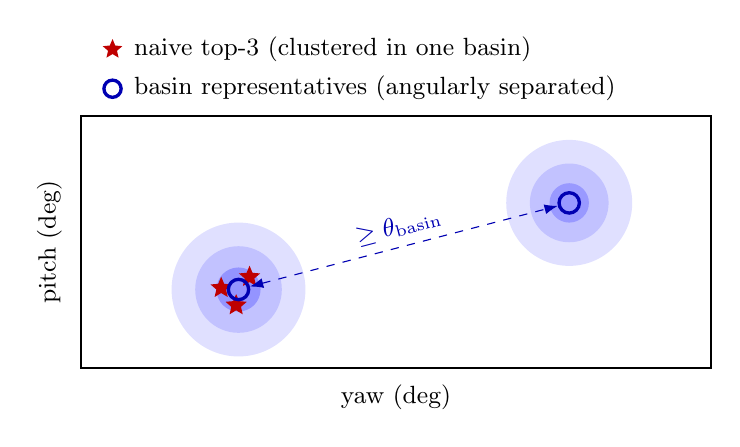
\begin{tikzpicture}[>=Latex, every node/.style={font=\small}]
  % yaw-pitch landscape frame
  \draw[thick] (0,0) rectangle (8,3.2);
  \node[below] at (4,-0.08) {yaw (deg)};
  \node[rotate=90, above] at (-0.12,1.6) {pitch (deg)};
  % low-cost basin A (lower-left) as concentric rings
  \foreach \rr/\op in {0.85/12, 0.55/24, 0.28/42}{\fill[blue!\op] (2.0,1.0) circle (\rr);}
  % low-cost basin B (upper-right)
  \foreach \rr/\op in {0.80/12, 0.50/24, 0.25/40}{\fill[blue!\op] (6.2,2.1) circle (\rr);}
  % naive top-3: three stars clustered inside basin A
  \foreach \p in {(1.78,1.02),(2.14,1.16),(1.97,0.80)}{
    \node[star, star points=5, star point ratio=2.2, fill=red!75!black, inner sep=1.3pt] at \p {};}
  % basin-NMS representatives: one per basin
  \node[circle, draw=blue!70!black, very thick, inner sep=2.6pt] (rA) at (2.0,1.0) {};
  \node[circle, draw=blue!70!black, very thick, inner sep=2.6pt] (rB) at (6.2,2.1) {};
  \draw[<->, blue!70!black, dashed] (rA) -- (rB) node[midway, above, sloped] {$\ge\theta_{\mathrm{basin}}$};
  % legend (above the frame), stacked on two rows so the long labels never overlap
  \node[star, star points=5, star point ratio=2.2, fill=red!75!black, inner sep=1.2pt] at (0.4,4.05) {};
  \node[right] at (0.55,4.05) {naive top-3 (clustered in one basin)};
  \node[circle, draw=blue!70!black, very thick, inner sep=2.2pt] at (0.4,3.55) {};
  \node[right] at (0.55,3.55) {basin representatives (angularly separated)};
\end{tikzpicture}
\caption{Top-$k$ points vs.\ Top-$k$ basins. When there are several mutually separated low-cost basins (blue regions) on the
yaw--pitch cost landscape, simply picking the top points with small $v_{ss}$ (red stars) repeatedly selects only neighboring points
within one basin. With angular non-maximum suppression (NMS), keeping only candidates that are at least $\theta_{\mathrm{basin}}$
away from the already-chosen representatives (blue circles), different near-optimal orientation groups are presented as representatives.}
\label{fig:basin-nms}
\end{figure}

Therefore, the current visualization and post-processing mark the top basins (top-$k$ basins) rather than the top points (top-$k$ points).
After converting a yaw--pitch point $(\psi,\phi)$ to a build direction $n(\psi,\phi)$,
the distance between two orientations is defined as
\begin{equation}
d(n_a,n_b)
=
\cos^{-1}(n_a\cdot n_b)
\end{equation}
Here we use $n_a\cdot n_b$ rather than $|n_a\cdot n_b|$.
This is because, in the yaw--pitch orientation of TOMO\_INT3, $n$ and $-n$ can represent different build orientations.
Scanning the sorted candidate list in order,
a candidate whose angular difference from an already-selected basin representative satisfies
\begin{equation}
d(n,n_r) < \theta_{\mathrm{basin}}
\end{equation}
is considered the same basin and removed.
The current implementation used $\theta_{\mathrm{basin}}=12^\circ$.

For the TOMO\_INT3 contour itself, after sorting the $v_{ss}$ grid in ascending or descending order,
we apply the angular non-maximum suppression%
\footnote{Non-maximum suppression (NMS): a technique that adopts candidates from the best-scoring one in turn, but removes candidates
too close to an already-adopted one to eliminate duplicates (originating from object detection). Here ``closeness'' is defined as the angle
between two orientations, to prevent neighboring directions of the same basin from being redundantly selected.}
above to select 3 optimal-basin representatives and 3 worst-basin representatives respectively.
This approach shows, when the global optimum exists in multiple places,
different optimal orientation groups instead of redundant grid points of the same basin.

The same basin perspective is applied to the SFTF candidates as well.
First, we sort candidates with low and high final tuning score $T(n)$ respectively, but
we remove same-basin duplicates to select low-score basin candidates and high-score basin candidates respectively.
The current implementation keeps up to 40 basin candidates per direction.
Then we put each candidate as the initial yaw--pitch orientation of TOMO\_INT3,
set the angle step to 0, and compute only a single orientation.
That is, for candidate $q_k=(yaw_k,pitch_k)$ we directly measure
\begin{equation}
\mathrm{Mss}_k
=
\mathrm{TOMO\_INT3}(q_k;\Delta\theta=0)
\end{equation}
Finally, we re-sort the candidate basins by this $\mathrm{Mss}_k$ value,
and mark the 3 with small measured Mss as measured optimal basins
and the 3 with large measured Mss as measured worst basins.

This procedure does not interpret the order of the SFTF scores directly as the final optimal/worst.
Instead, SFTF plays the role of quickly proposing a broad candidate basin,
and TOMO\_INT3 is used as an accurate single-orientation verifier for a small number of candidates.
Therefore the user can confirm not only a single optimal orientation, but
several orientation groups that are mutually separated yet have a small actual support mass.
This is especially useful when, in build orientation optimization, ``which selectable optimal orientation groups exist''
is more important than the coordinates of the rank-1 itself.

In an additional analysis, we mapped all coarse/refined candidates onto the TOMO grid to check the lowest $v_{ss}$ within the candidate pool.
With the default $512$ coarse directions, the candidate pool of happy 50k itself did not sufficiently include the vicinity of the TOMO optimum.
Increasing the number of coarse directions to $2048$ lowered the lowest ratio within the candidate pool of happy 50k to about $1.91$.
This means that the failure of happy 50k is not merely a score tuning problem, but
also includes limitations of the direction-sampling resolution and the candidate-generation method.
However, in the $2048$-candidate pool there was difficulty in stably selecting a good candidate with the current features alone.
Good candidates were generally located in an intermediate region where the build-plate penalty is low while
the pair flow and hit count are not too low.
Therefore, in the future, rather than a simple linear rank score,
a feature that directly reflects the face-to-face self-support coverage or a TOMO-style support-volume proxy is needed.

The main improvement factors confirmed in this experiment are as follows.

\begin{itemize}
\item The sign of the overhang normal and the build direction sign were directly reflected.
\item Face-to-face internal visibility was evaluated via ray casting.
\item A valid receiver face condition was imposed to consider only actually supportable faces.
\item Overhangs that must be directly supported all the way to the build plate were handled as a separate penalty.
\item Instead of 3 eigenaxes, spherical sampling and local re-search were used.
\item In the final candidate selection, rank-normalized feature tuning based on comparison with the TOMO\_INT3 grid was applied.
\item In the final visualization, angularly separated top-$k$ basin representatives were marked rather than top-$k$ points,
providing the user with different near-optimal orientation groups.
\end{itemize}

At the same time, these results suggest that the current SFTF is useful not so much as a complete replacement of the TOMO\_INT3 optimum,
but as a candidate generator or warm-start method for reducing the expensive yaw--pitch global search.
In particular, after proposing a few top candidates,
locally verifying only their vicinity with TOMO or a slicer can greatly reduce the overall search cost.

\section{Method Analysis: Feature Contribution, Cross-Validation, Comparison with Existing Methods}

In this section we quantitatively analyze the validity of the proposed method from three perspectives.
All analyses reuse the stored $1^\circ$ TOMO\_INT3 $v_{ss}$ grid and do not require GPU recomputation,
and are reproducible with the public analysis scripts.
Unless otherwise noted, the best-of-3 ratio is the ratio, relative to the TOMO global optimum, of the smallest signed $v_{ss}$
among the top 3 candidates ($3^\circ$ angular NMS) when mapped onto the TOMO grid, and smaller is better.

\subsection{Feature Correlation and Objective Function Ablation}
\label{sec:ablation}

First, how much each feature predicts the actual $v_{ss}$ was evaluated by the
feature--$v_{ss}$ Spearman rank correlation%
\footnote{Spearman rank correlation coefficient: a correlation computed after converting two variables into \emph{ranks} instead of values,
where $+1$ means a perfectly monotonically increasing relationship and $-1$ a perfectly monotonically decreasing one. It measures whether
``large values go together and small values go together'' even if the relationship is not linear. See: \cite{spearman1904}}
over the entire candidate pool (Table~\ref{tab:feature-corr}).

\begin{table}[H]
\centering
\caption{Spearman rank correlation between features and TOMO $v_{ss}$ over the entire candidate pool.
The larger the positive value, the more valid the feature is as a cost.}
\label{tab:feature-corr}
\begin{tabular}{lrrrrrr}
\toprule
Feature & Bunny & manikin & dragon & happy & lucy & Average\\
\midrule
$J=R{+}P{+}B$         & 0.46 & 0.26 & 0.80 & 0.27 & 0.57 & 0.47\\
$R$ (Rayleigh)        & 0.40 & $-0.33$ & $-0.57$ & $-0.03$ & 0.14 & $-0.08$\\
$P$ (pair flow)       & $-0.04$ & $-0.38$ & $-0.72$ & 0.00 & $-0.59$ & $-0.34$\\
$B$ (build-plate)     & \textbf{0.50} & \textbf{0.66} & \textbf{0.85} & \textbf{0.29} & \textbf{0.62} & \textbf{0.58}\\
$H$ (hit count)       & 0.24 & $-0.53$ & $-0.73$ & $-0.00$ & $-0.71$ & $-0.35$\\
$S$ (nuclear)         & $-0.02$ & $-0.36$ & $-0.70$ & $-0.05$ & $-0.26$ & $-0.28$\\
$\sigma_1$            & $-0.03$ & $-0.34$ & $-0.66$ & $-0.07$ & 0.07 & $-0.21$\\
\bottomrule
\end{tabular}
\end{table}

Only the build-plate term $B(n)$ has a consistent positive correlation across all meshes ($0.29$--$0.85$, average $0.58$),
even higher than the predictive power of the entire objective function $J$ (average $0.47$).
By contrast, $P$, $S$, $\sigma_1$ derived from the asymmetric tensor and the hit count $H$ have negative average correlations
and flip sign from mesh to mesh. That is, these terms do not generalize as cost terms with a fixed sign.

To re-confirm this at the objective-function level, we sorted candidates by several objective-function variants and then
measured the best-of-3 ratio (Table~\ref{tab:ablation}).

\begin{table}[H]
\centering
\caption{Best-of-3 ratio of the objective-function ablation (lower is better).
The proposed objective function $J=R+P+B$ and the old objective function including nuclear/$\sigma_1$ are completely identical per mesh.}
\label{tab:ablation}
\begin{tabular}{lrrrrrr}
\toprule
Ranking variant & Bunny & manikin & dragon & happy & lucy & Average\\
\midrule
$T$ (rank tuned, in-sample) & 1.46 & 1.86 & 1.62 & 11.23 & 2.82 & 3.80\\
$J=R+P+B$ (proposed)            & 2.47 & 3.99 & 2.01 & 11.15 & 2.82 & 4.49\\
$R{+}P{+}B{+}0.05S{+}0.05\sigma_1$ (old objective) & 2.47 & 3.99 & 2.01 & 11.15 & 2.82 & 4.49\\
$B$ alone                     & 2.57 & 2.60 & 1.94 & 16.04 & 2.82 & 5.19\\
$0.05S+0.05\sigma_1$ (tensor alone) & 5.82 & 5.38 & 6.57 & 11.86 & 5.62 & 7.05\\
$P$ alone                     & 5.82 & 4.92 & 6.27 & 12.07 & 7.51 & 7.32\\
\bottomrule
\end{tabular}
\end{table}

Crucially, the results of the proposed objective function $J=R+P+B$ and the old objective function including the nuclear/$\sigma_1$ terms are identical across all meshes.
This means that the nuclear/$\sigma_1$ terms with weight $0.05$ essentially do not contribute to the final candidate selection,
and is the basis for excluding these terms from the objective function in this revision.
Also, the variants using only tensor-derived terms ($0.05S+0.05\sigma_1$, $P$ alone) have the worst ratios.
That is, the predictive power of our method originates not from the asymmetric tensor structure but from the build-plate penalty and the internal visibility evaluation,
and the tensor terms play only an auxiliary role.

\subsection{Reformulation into a Unified Tensor: Rayleigh Equivalence of the Build-Plate Term}
\label{sec:unified}

The ablation in \S\ref{sec:ablation} showed that the build-plate term $B$ takes almost full charge of the predictive power
and that the Rayleigh term $R$ derived from the tensor flips sign from mesh to mesh (Table~\ref{tab:feature-corr}).
However, according to the virtual ground node interpretation of \S\ref{sec:groundnode}, $B$ itself is a Rayleigh contribution of the augmented flow tensor,
and the unified Rayleigh cost is exactly expressed as $\tilde R=R+B$ (Eq.~\eqref{eq:Rtilde}).
This section verifies whether that unified term is actually a better predictor.

First, we confirmed the equivalence numerically.
Computing the Rayleigh cost of the augmented tensor $\tilde F(n)$ directly over the entire candidate pool of the five stored meshes,
it was identical within floating-point error, with $|\tilde R-(R+B)|<10^{-12}$ for all candidates.

Table~\ref{tab:unified-corr} compares the Spearman correlation of the unified term $\tilde R$ with the single terms.
With $R$ alone the average is $-0.08$ (unstable sign), but
$\tilde R=R+B$ with the ground node added has an average of $0.60$, the best among single features,
even higher than the current objective function $J=R+P+B$ (average $0.47$).
The reason $J$ is lower than $\tilde R$ is that the face-to-face support volume $P$ (average correlation $-0.34$, Table~\ref{tab:feature-corr})
acts as a negative signal and lowers the predictive power when summed.

\begin{table}[H]
\centering
\caption{Spearman correlation of the unified Rayleigh term $\tilde R=R+B$ and single terms with TOMO $v_{ss}$ (higher is better).
$\tilde R$ was computed directly from the augmented tensor and agrees with $R+B$ within $10^{-12}$.}
\label{tab:unified-corr}
\begin{tabular}{lrrrr}
\toprule
Mesh & $R$ & $B$ & $\tilde R=R{+}B$ & $J=R{+}P{+}B$\\
\midrule
Bunny   & 0.40 & 0.50 & \textbf{0.52} & 0.46\\
manikin & $-0.33$ & 0.66 & 0.65 & 0.26\\
dragon  & $-0.57$ & 0.85 & \textbf{0.89} & 0.80\\
happy   & $-0.03$ & 0.29 & \textbf{0.31} & 0.27\\
lucy    & 0.14 & 0.62 & 0.62 & 0.57\\
\midrule
Average    & $-0.08$ & 0.58 & \textbf{0.60} & 0.47\\
\bottomrule
\end{tabular}
\end{table}

This was also confirmed by the best-of-3 ratio (Table~\ref{tab:unified-b3}).
Sorting candidates by the unified term alone (i.e., removing $P$),
the average ratio over the 4 meshes with normal candidate generation improves from $J$'s $2.82$ to $\tilde R$'s $2.50$.
happy is a separate case where the candidate pool itself does not include a near-optimal (\S\ref{sec:robustness}),
and on this mesh the unified term is rather worse, but this is due to a sampling limitation, not scoring.

\begin{table}[H]
\centering
\caption{Best-of-3 ratio when sorting candidates by $J=R+P+B$ and the unified term $\tilde R=R+B$ (lower is better).
On the average excluding happy (candidate generation failure, \S\ref{sec:robustness}), $\tilde R$ outperforms $J$.}
\label{tab:unified-b3}
\begin{tabular}{lrr}
\toprule
Mesh & $J=R{+}P{+}B$ & $\tilde R=R{+}B$\\
\midrule
Bunny   & \textbf{2.47} & 2.57\\
manikin & 3.99 & \textbf{2.89}\\
dragon  & 2.01 & \textbf{1.70}\\
lucy    & 2.82 & 2.82\\
\midrule
Average (excl.\ happy) & 2.82 & \textbf{2.50}\\
\bottomrule
\end{tabular}
\end{table}

In summary, the unified tensor reformulation (i) formulates the build-plate cost as a term of the flow tensor,
justifying the ``tensor'' representation, and (ii) shows that the single-tensor Rayleigh cost $\tilde R$ with the negative signal $P$ removed
is consistently superior to the existing $J$.

\paragraph{Verification of the Height Convention.}
The ground term uses a height convention opposite in sign to the face-to-face term (amplification instead of attenuation).
To show that this asymmetry is not arbitrary, we compared four plate conventions.
The current amplification $B_{\mathrm{amp}}=\sum O_iA_i(1+\alpha h)$,
the height-free $B_{\mathrm{flat}}=\sum O_iA_i$,
the attenuation $B_{\mathrm{att}}=\sum O_iA_i/(1+\alpha h)$ symmetric with the face-to-face term,
and $B_{\mathrm{uni}}=\sum O_i^2A_i/(1+\alpha h)$ that fully follows the face-to-face weight law.
The average Spearman correlations were $0.58$, $0.51$, $0.43$, $0.47$ respectively,
so \emph{the current amplification convention is the highest and most consistent},
and the attenuation convention $B_{\mathrm{att}}$ matched symmetrically with the face-to-face term was the lowest (negative correlation on happy).
That is, the sign asymmetry ``distant self-support is weakened, tall build-plate support is strengthened''
is physically correct and empirically supported.
However, the fully unified convention $B_{\mathrm{uni}}$ greatly improves best-of-3 on slender shapes such as manikin
(e.g., manikin $2.89\to1.37$), leaving room for a shape-adaptive convention in the future.

\subsection{Cross-Validation of Rank Tuning}
\label{sec:cv}

Since the rank tuning weights in Table~\ref{tab:sftf-tomo-comparison} were calibrated together on the reported meshes,
to evaluate generalization performance we performed Leave-One-Mesh-Out (LOMO) cross-validation.%
\footnote{Cross-validation: a method that sets aside part of the data from training and uses it only for validation, to estimate performance
on unseen data. LOMO is a ``leave one mesh out'' scheme that excludes one mesh, fits the weights on the rest, and then measures performance
on the excluded mesh. See: \cite{stone1974}}
Setting each mesh as hold-out and refitting the weights on the remaining meshes
(ridge regression%
\footnote{Ridge regression: linear regression that adds an $L_2$ penalty so that the regression weights do not become too large,
reducing overfitting. See: \cite{hoerl1970}} on the intra-mesh rank-normalized features, with the target being the intra-mesh rank-normalized $v_{ss}$),
we measured the best-of-3 ratio of the hold-out mesh.
Excluding happy, for which candidate generation itself fails (see the end of \S\ref{sec:cv} below and the oracle),
we evaluated on the 4 meshes whose candidate pool includes a near-optimal direction.

\begin{table}[H]
\centering
\caption{LOMO cross-validation best-of-3 ratio of rank tuning (lower is better).
The in-sample column is the calibration-set fit value reported in Table~\ref{tab:sftf-tomo-comparison}.
The oracle is the best direction existing within the candidate pool, representing the upper bound of candidate generation.}
\label{tab:lomo-cv}
\begin{tabular}{lrrrr}
\toprule
Mesh & oracle & untuned $J$ & in-sample (reported) & LOMO\\
\midrule
Bunny    & 1.46 & 2.47 & 1.46 & 2.20\\
manikin  & 1.13 & 3.99 & 1.86 & 2.62\\
dragon   & 1.29 & 2.01 & 1.62 & 1.86\\
lucy     & 1.02 & 2.82 & 2.82 & 2.82\\
\midrule
Average     & 1.22 & 2.82 & \textbf{1.94} & \textbf{2.37}\\
\bottomrule
\end{tabular}
\end{table}

The reported in-sample average $1.94$ is not reproduced in honest cross-validation,
and the hold-out average is $2.37$, about $0.43$ (about $22\%$) higher. This difference is the optimistic bias of the weight calibration.
Also, among the 7 weights, only $R$ ($\approx 0.7$) and $B$ ($\approx 1.0$) are reproduced stably across folds,
while the reported large $P=-2.39$, $H=2.31$, $S=-2.29$, $\sigma_1=1.64$ are not reproduced in any fold.
In fact, the LOMO average ratio of reduced models using only stable features is
$B$ alone $2.48$, $R+B$ $2.46$, $R+P+B$ $2.44$, not much different from the full 7-feature model ($2.37$),
and all are superior to untuned $J$ ($2.82$).
Therefore, instead of 7 calibrated weights, tuning a few features centered on $R$, $B$ (and $P$ if needed) is simpler yet more robust.
Meanwhile, the fact that the hold-out ratio is clearly larger than the oracle ($1.22$) in all variants suggests
that the room for improvement lies not in candidate generation but in the scoring stage.

\subsection{Unified Comparison with Existing Methods}
\label{sec:baseline}

Finally, under the same best-of-3 ratio criterion we compared PCA directions, Support Tensor eigenvector directions,
and SFTF (untuned and LOMO cross-validation tuned) (Table~\ref{tab:unified}).
PCA
uses the principal axes of the area-weighted face-centroid covariance, and Support Tensor uses the eigenvectors of $M=\sum_i A_i m_i m_i^T$,
taking the best value over the 3 axes of each method (including $\pm$).
The SFTF-tuned column is not an in-sample value but the LOMO value of \S\ref{sec:cv}.

\begin{table}[H]
\centering
\caption{Unified comparison of existing methods and SFTF (best-of-3 signed $v_{ss}$ ratio, lower is better).
SFTF-tuned is the cross-validated generalization estimate.}
\label{tab:unified}
\begin{tabular}{lrrrrr}
\toprule
Mesh & PCA & Support Tensor & SFTF untuned & SFTF tuned (LOMO) & oracle\\
\midrule
Bunny    & 2.82 & 3.71 & 2.47 & 2.20 & 1.46\\
manikin  & 2.65 & 2.50 & 3.99 & 2.62 & 1.13\\
dragon   & 2.69 & 2.33 & 2.01 & 1.86 & 1.29\\
lucy     & 6.37 & 8.67 & 2.82 & 2.82 & 1.02\\
\midrule
Average     & 3.63 & 4.30 & 2.82 & \textbf{2.37} & 1.22\\
\bottomrule
\end{tabular}
\end{table}

Cross-validated SFTF (average $2.37$) is about $35\%$ better than PCA ($3.63$) and about $45\%$ better than Support Tensor eigenvectors ($4.30$),
and even untuned $J$ ($2.82$) is better than the two existing methods.
In particular, the Support Tensor eigenvectors are worse than even PCA ($8.67$ on lucy),
which quantitatively supports this study's starting assumption that the statistical principal axes of the normal distribution alone
cannot explain the direction-dependent support volume.
This comparison shows that even when discarding the reported in-sample numbers and using the conservative cross-validation numbers,
SFTF's advantage over existing methods is maintained.

\subsection{Additional Robustness Analysis: Critical Angle, Sampling Density, Dimensional Normalization}
\label{sec:robustness}

\paragraph{Critical Angle Matching.}
SFTF's overhang definition $O_i(n)=\max(0,-m_i\cdot n)$ includes all downward faces regardless of the critical angle, but
TOMO\_INT3 regards as support-needing only the faces with $-m_i\cdot n>\cos\theta_c$ among downward faces ($m_i\cdot n<0$).
As a result of applying the same gate to the SFTF overhang to match the definitions,
under the $\theta_c=60^\circ$ setting (same as TOMO) the LOMO average best-of-3 ratio
worsened from $2.37$ to $2.82$, and at $\theta_c=45^\circ$ it was $2.42$, similar to the baseline.
That is, matching the critical angle gate does not provide a consistent improvement,
which is interpreted as the rank tuning already absorbing the difference in the overhang definition.
Therefore the default implementation does not apply the gate.

\paragraph{Sampling Density and Candidate Generation Limit.}
Increasing the number of coarse Fibonacci sphere directions, we measured the best value within the candidate pool (oracle ratio) (Table~\ref{tab:sampling}).

\begin{table}[H]
\centering
\caption{Oracle (best within candidate pool) ratio by the number of coarse directions. Meshes other than happy
already include a near-optimal direction at $512$.}
\label{tab:sampling}
\begin{tabular}{rrrrrr}
\toprule
\# coarse directions & Bunny & manikin & dragon & happy & lucy\\
\midrule
512  & 1.46 & 1.13 & 1.29 & 4.35 & 1.02\\
1024 & 1.50 & 1.11 & 1.33 & 3.94 & 1.02\\
2048 & 1.61 & 1.06 & 1.28 & \textbf{1.91} & 1.04\\
4096 & 1.62 & 1.13 & 1.27 & 1.91 & 1.30\\
\bottomrule
\end{tabular}
\end{table}

happy's oracle ratio is $4.35$ at $512$, with no near-optimal direction included in the candidate pool.
Increasing the number of directions to $2048$ lowers it to $1.91$, partially resolving the candidate-generation limit.
By contrast, other meshes already have an oracle of $1.0$--$1.5$ at $512$, with no benefit from increasing the number of directions.
However, even when its candidates are reinforced, happy's best-of-3 ratio of untuned $J$ remains at $10.51$ even at $4096$,
showing limitations in both sampling and scoring. This is the basis for separating happy as a distinct hard case.

\paragraph{Dimensional Normalization of the Objective Function.}
The terms of the objective function $J=R+P+B$ have different units ($R,P\sim$ area$^2$, $B\sim$ area).
When the three terms are normalized to the same scale within the candidate pool and summed with equal weights,
the Spearman correlation of raw $J$ drops greatly from $0.52$ to $0.14$ under min--max normalization%
\footnote{Feature scaling (normalization) that linearly maps the minimum to 0 and the maximum to 1. See: \cite{hanmining}}
and to $0.10$ under z-score normalization,%
\footnote{Standard score. A normalization that subtracts the mean and divides by the standard deviation to make ``mean 0, variance 1.''
See: \cite{hanmining}}
and the best-of-3 ratio also worsens from $2.82$ to $3.53$ and $3.86$ respectively.
This shows that the predictive power of raw $J$ originates not from a balance of several terms but from the dominance of the build-plate term, which has the largest scale.
Therefore the physical meaning of the weights is more properly secured not by simple dimensional normalization,
but by removing non-predictive terms and reducing to a focus on $R$, $B$ (\S\ref{sec:cv}).

\section{Verification against Four Implementations on a Controlled Five-Group Shape Set}
\label{sec:fivegroup}

While the preceding sections addressed the accuracy and generalization on stored Stanford mesh grids,
this section directly contrasts SFTF's \emph{algorithmic characteristics} on a difficulty-controlled shape set
with the four implementations TOMO\_INT3, TOMO\_CUDA, Python SFTF, and SFTF\_C++.
The verification was performed as a batch experiment;
SFTF generates a candidate pool from the input mesh alone (coarse $512$ directions, candidate pool $1292$),
while TOMO\_INT3 and TOMO\_CUDA performed an exhaustive sweep on the same mesh over a yaw--pitch $3^\circ$ grid
($120\times120=14{,}400$ directions), critical angle $60^\circ$, via DLL.%
\footnote{To handle a large-scale batch that sweeps $35$ meshes over $5$ critical angles ($\theta_c\in\{0,30,45,60,90\}^\circ$) with two backends,
the sweep grid of this verification was set to a coarser $3^\circ$ than the prior GPU-MSST's $1^\circ$
($360\times360=129{,}600$ directions). On a denser $1^\circ$ grid, the TOMO sweep time increases about $9\times$, widening the speed gap relative to SFTF further.}
SFTF\_C++ is an implementation that ports the same candidate-generation algorithm as Python SFTF to a C++ DLL,
and the measured value is the pure computation time of the candidate generator.
All four implementation times are available for all $35$ meshes A--E.

\subsection{Experimental Setup}

The dataset consists of five groups that deliberately separate and control the two axes of \emph{shape difficulty} and \emph{mesh scale}.
A--C set the scale in the $\sim$$10^1$--$10^5$-face range and vary the difficulty axis from basic shapes to freeform organic shapes,
revealing the \emph{fixed-cost floor} of the exhaustive sweep (a cost almost independent of mesh complexity).
D--E fix the difficulty as real manufacturing parts while pushing the scale axis from $256$ faces to $1.04\times10^6$ faces,
revealing the \emph{adaptive cost} by which the SFTF candidate-evaluation cost increases adaptively to mesh complexity.
Therefore A--E is not a single size ramp, and the partial overlap of the face-count ranges of groups C and D
is the result of a design that separates and controls the two axes, not an ordering error.
\begin{itemize}
\item \textbf{A (basic shapes, 5; lower difficulty)}: cube, sphere, cylinder, cone, torus (face count $\sim$$10^1$--$10^3$).
\item \textbf{B (simple functional parts, 5; mid difficulty)}: u\_bracket, hook, c\_clamp, pipe\_elbow, hollow\_box.
\item \textbf{C (organic/freeform benchmarks, 5; upper difficulty)}: standard scan/sculpture meshes such as Bunny ($69{,}662$ faces), manikin, dragon ($\sim$$10^5$ faces), happy, lucy. The Stanford grid meshes of the preceding sections are exactly this group.
\item \textbf{D (Thingi10K set 1, 10; lower scale)}: real manufacturing parts with $256$--$88{,}106$ faces~\cite{Thingi10K}.
\item \textbf{E (Thingi10K set 2, 10; upper scale)}: large high-resolution meshes with about $5.1\times10^5$--$1.04\times10^6$ faces.
\end{itemize}
For the $35$ meshes A--E, we recorded the Python SFTF candidate-evaluation time,
the TOMO\_INT3 DLL sweep time, the TOMO\_CUDA DLL sweep time, the SFTF\_C++ candidate-evaluation time,
the hit count and candidate score of the SFTF top direction, and the TOMO contour HTML.
This section addresses the contrast of computational structure and implementation axes rather than the direction-accuracy ratio,
and the quantitative analysis of direction accuracy is handled by the grid comparison of \S\ref{sec:ablation}--\S\ref{sec:baseline}.

\subsection{Overall Computation Time Comparison}

Table~\ref{tab:fivegroup-timing} summarizes the four-implementation measurements of the $35$ meshes.
The most prominent characteristic is the contrast of \emph{fixed cost vs.\ adaptive cost}.
TOMO\_INT3 takes about $4$ seconds even for a cube with only $12$ faces,
having a large fixed cost almost independent of mesh complexity due to the nature of the yaw--pitch exhaustive sweep (because even on a $3^\circ$ grid it evaluates all $14{,}400$ directions).
By contrast, the cost of SFTF adapts to mesh complexity,
remaining $0.12$--$0.74$ seconds for basic shapes, $1.0$--$3.2$ seconds for organic benchmarks (C),
$0.36$--$3.42$ seconds for Thingi10K parts (D), and only $9.71$--$22.11$ seconds even for large meshes of $500$k--$1$M faces (E).
Over all $35$, Python SFTF is $1.4$--$34\times$ faster than TOMO\_INT3 ($3^\circ$),
with an average speed ratio of about $9\times$.
SFTF\_C++ is additionally $3.9$--$233\times$ faster than Python SFTF,
and $10$--$5{,}160\times$ faster than TOMO\_INT3 ($3^\circ$).
That is, SFTF is suitable not as a replacement for the expensive global sweep, but
as a candidate generator that proposes promising orientations from several to several thousand times faster in front of it,
and the denser the sweep grid is made to $1^\circ$, the wider this gap becomes.

The result of TOMO\_CUDA is more subtle.
On the simple shapes of A/B, TOMO\_CUDA is generally faster than TOMO\_INT3
and shows the GPU-acceleration effect of the exhaustive sweep.
However, on the organic and large meshes of C/D/E, TOMO\_CUDA is often slower than TOMO\_INT3,
and on the overall average the TOMO\_CUDA/TOMO\_INT3 time ratio is about $1.07$.
This means that in this verification environment, the input preparation of the exhaustive sweep, the mesh complexity,
and the DLL-internal data structures and memory-movement cost can govern performance more than the GPU backend itself.
Therefore the core speed gain of this paper comes not from the ``hardware axis of changing INT3 to CUDA''
but from the ``algorithmic axis of reducing $14{,}400$ exhaustive directions on a $3^\circ$ grid ($129{,}600$ at $1^\circ$) to a $1292$-candidate evaluation.''

\begin{table}[H]
\footnotesize
\centering
\caption{Computation time of the four implementations for the $35$ meshes of the five groups.
$t_{\mathrm{INT3}}$ and $t_{\mathrm{CUDA}}$ are the TOMO\_INT3/TOMO\_CUDA $3^\circ$ exhaustive sweep ($\theta_c=60^\circ$) DLL times respectively,
$t_{\mathrm{py}}$ is the Python SFTF candidate evaluation, and $t_{\mathrm{C++}}$ is the SFTF\_C++ pure computation time.
hit is the number of valid face-to-face supports of the Python SFTF top direction.
The speed columns are $t_{\mathrm{INT3}}/t_{\mathrm{py}}$ and $t_{\mathrm{INT3}}/t_{\mathrm{C++}}$ respectively.}
\label{tab:fivegroup-timing}
\resizebox{\textwidth}{!}{%
\begin{tabular}{llrrrrrrrr}
\toprule
ID & Shape & Faces & hit & $t_{\mathrm{INT3}}$(s) & $t_{\mathrm{CUDA}}$(s) & $t_{\mathrm{py}}$(s) & $t_{\mathrm{C++}}$(ms) & INT3/py & INT3/C++\\
\midrule
\multicolumn{10}{l}{\textit{A: basic shapes}}\\
A1 & cube        & 12     & 0   & 4.12 & 1.26 & 0.13 & 4.1    & $32\times$  & $1{,}006\times$\\
A2 & sphere      & 2{,}976  & 498 & 4.29 & 1.53 & 0.74 & 23.9   & $6\times$   & $179\times$\\
A3 & cylinder    & 192    & 0   & 4.12 & 2.16 & 0.17 & 1.3    & $24\times$  & $3{,}172\times$\\
A4 & cone        & 96     & 0   & 4.13 & 1.47 & 0.12 & 0.8    & $34\times$  & $5{,}157\times$\\
A5 & torus       & 2{,}304  & 184 & 4.28 & 1.48 & 0.45 & 14.2   & $10\times$  & $301\times$\\
\midrule
\multicolumn{10}{l}{\textit{B: simple parts}}\\
B1 & u\_bracket   & 28     & 2   & 4.13 & 1.35 & 0.15 & 3.9    & $28\times$  & $1{,}059\times$\\
B2 & hook        & 1{,}560  & 235 & 4.21 & 1.44 & 0.58 & 15.8   & $7\times$   & $266\times$\\
B3 & c\_clamp     & 28     & 1   & 4.13 & 1.63 & 0.17 & 0.8    & $24\times$  & $5{,}157\times$\\
B4 & pipe\_elbow  & 2{,}400  & 500 & 4.27 & 1.49 & 0.81 & 25.3   & $5\times$   & $169\times$\\
B5 & hollow\_box  & 24     & 4   & 4.13 & 1.64 & 0.21 & 0.9    & $20\times$  & $4{,}592\times$\\
\midrule
\multicolumn{10}{l}{\textit{C: organic benchmarks}}\\
C1 & Bunny       & 69{,}662 & 81  & 6.17  & 6.97  & 1.69 & 247.7 & $4\times$  & $25\times$\\
C2 & manikin     & 13{,}672 & 134 & 4.38  & 3.70  & 1.02 & 44.3  & $4\times$  & $99\times$\\
C3 & dragon      & 99{,}999 & 970 & 9.65  & 12.11 & 3.17 & 323.3 & $3\times$  & $30\times$\\
C4 & happy       & 49{,}944 & 240 & 5.92  & 6.63  & 1.50 & 130.1 & $4\times$  & $45\times$\\
C5 & lucy        & 49{,}999 & 542 & 6.44  & 8.87  & 1.87 & 172.5 & $3\times$  & $37\times$\\
\midrule
\multicolumn{10}{l}{\textit{D: Thingi10K set 1}}\\
D1  & 37009 & 23{,}909 & 57  & 5.76  & 13.28 & 1.37 & 114.5 & $4\times$   & $50\times$\\
D2  & 37010 & 13{,}247 & 35  & 4.95  & 13.28 & 1.24 & 63.5  & $4\times$   & $78\times$\\
D3  & 37011 & 17{,}288 & 82  & 5.06  & 5.81  & 1.15 & 89.2  & $4\times$   & $57\times$\\
D4  & 37091 & 256    & 42  & 4.13  & 2.00  & 0.36 & 5.2   & $11\times$  & $795\times$\\
D5  & 37095 & 468    & 65  & 4.17  & 3.62  & 0.49 & 6.2   & $9\times$   & $672\times$\\
D6  & 37111 & 88{,}106 & 386 & 12.33 & 21.37 & 3.42 & 465.4 & $4\times$   & $26\times$\\
D7  & 37137 & 64{,}078 & 434 & 10.18 & 22.16 & 2.90 & 305.5 & $4\times$   & $33\times$\\
D8  & 37402 & 8{,}322  & 119 & 5.00  & 6.82  & 2.43 & 49.7  & $2\times$   & $101\times$\\
D9  & 37415 & 13{,}340 & 77  & 5.73  & 11.52 & 2.96 & 65.4  & $2\times$   & $88\times$\\
D10 & 37416 & 12{,}036 & 496 & 4.74  & 6.10  & 3.39 & 80.4  & $1.4\times$ & $59\times$\\
\midrule
\multicolumn{10}{l}{\textit{E: Thingi10K set 2, large meshes}}\\
E1  & 39507 & 969{,}520   & 562   & 129.39 & 131.73 & 16.92 & 4387.6 & $8\times$   & $29\times$\\
E2  & 45809 & 517{,}589   & 107   & 64.89  & 73.88  & 9.71  & 1984.5 & $7\times$   & $33\times$\\
E3  & 45811 & 1{,}037{,}876 & 1{,}309 & 132.74 & 145.57 & 18.69 & 4515.6 & $7\times$   & $29\times$\\
E4  & 46012 & 638{,}754   & 50    & 82.74  & 101.35 & 11.15 & 2583.8 & $7\times$   & $32\times$\\
E5  & 55280 & 900{,}490   & 1{,}072 & 118.42 & 138.23 & 16.78 & 3957.9 & $7\times$   & $30\times$\\
E6  & 59197 & 786{,}432   & 699   & 99.04  & 105.32 & 17.50 & 4119.5 & $6\times$   & $24\times$\\
E7  & 61384 & 516{,}608   & 1{,}766 & 65.83  & 80.09  & 12.85 & 2065.0 & $5\times$   & $32\times$\\
E8  & 64445 & 514{,}938   & 2{,}288 & 21.98  & 31.69  & 15.05 & 2208.0 & $1.5\times$ & $10\times$\\
E9  & 64446 & 514{,}938   & 2{,}288 & 21.89  & 31.78  & 14.93 & 2211.4 & $1.5\times$ & $10\times$\\
E10 & 65942 & 754{,}688   & 1{,}175 & 108.07 & 111.99 & 22.11 & 3201.6 & $5\times$   & $34\times$\\
\bottomrule
\end{tabular}
}
\end{table}

\subsection{Group-wise Averages and Separation of Implementation Axes}
\label{sec:impl-compare}

\begin{table}[H]
\footnotesize
\centering
\caption{Group-wise average execution time and speed ratio.
The SFTF\_C++ average is in ms, and the rest are in seconds.
A TOMO\_CUDA/TOMO\_INT3 ratio greater than $1$ indicates a case where the CUDA backend is slower than INT3.}
\label{tab:fivegroup-impl}
\begin{tabular}{lrrrrrr}
\toprule
Group & py (s) & INT3 (s) & CUDA (s) & C++ (ms) & INT3/py & CUDA/INT3\\
\midrule
A & 0.32 & 4.19  & 1.58  & 8.9    & $6$--$34\times$   & $0.31$--$0.52$\\
B & 0.38 & 4.17  & 1.51  & 9.3    & $5$--$28\times$   & $0.33$--$0.40$\\
C & 1.85 & 6.51  & 7.66  & 183.6  & $3$--$4\times$    & $0.84$--$1.38$\\
D & 2.17 & 6.21  & 10.60 & 124.5  & $1.4$--$11\times$ & $0.48$--$2.68$\\
E & 15.57 & 84.50 & 95.16 & 3123.5 & $1.5$--$8\times$  & $1.02$--$1.45$\\
\bottomrule
\end{tabular}
\end{table}

\subsection{Scalability to Large Meshes (Group E)}
\label{sec:groupE}

Group E consists of $10$ large Thingi10K meshes with face counts from about $5.1\times10^5$ to $1.04\times10^6$,
examining whether SFTF works on high-resolution meshes beyond real-part scale.
The key observation is the \emph{gentle increase of the SFTF cost}.
Even on E meshes whose face count is about $6$--$12\times$ that of D6 ($88{,}106$ faces), Python SFTF candidate evaluation is $9.71$--$22.11$ seconds,
increasing only roughly sub-linearly with the face count.
This is because the ray budget is fixed at an upper bound of $3000$ via $K_{ray}=\mathrm{clip}(0.02N_f,500,3000)$,
so on large meshes the face preprocessing and BVH construction govern the cost while the ray casting cost saturates.
SFTF\_C++ finishes candidate evaluation on the same large meshes in $1.98$--$4.52$ seconds,
$3.9$--$6.9\times$ faster than Python.
These two candidate-generator costs are independent of the sweep grid (SFTF does not perform an exhaustive sweep).

By contrast, the $3^\circ$ exhaustive sweep of TOMO\_INT3 takes $22$--$133$ seconds on group E (about $9\times$, $126$--$1{,}077$ seconds, at $1^\circ$).
There are relatively short cases of about $22$ seconds on identical $514{,}938$-face meshes such as E8/E9, but
on most large meshes tens of seconds to over a hundred seconds are needed.
TOMO\_CUDA was also $32$--$146$ seconds, and was not faster than INT3 on large meshes in this verification environment.
This shows that the algorithmic reduction of the number of candidates provides a more stable speed gain even on large meshes
than the hardware acceleration of the exhaustive-sweep backend.

Internal consistency is also confirmed.
E8 ($64445$) and E9 ($64446$) are essentially identical meshes ($514{,}938$ faces),
and SFTF produced the same top score ($-0.9824$), the same direction, and the same hits ($2{,}288$),
showing deterministic reproducibility, with the only difference being the execution time ($15.05$ vs.\ $14.93$ seconds).
Also, the number of valid face-to-face supports (hit) increases as the mesh detail becomes richer
(e.g., E7 $1{,}766$, E8/E9 $2{,}288$), suggesting that the internal self-support structure of high-resolution shapes
is faithfully reflected in SFTF's flow tensor.

\subsection{Per-Direction Cost Structure Decomposition}

Unlike TOMO\_INT3, which summarizes each orientation with a single scalar $v_{ss}$,
SFTF provides the cost of the top direction decomposed into the Rayleigh term $R$, the face-to-face support volume $P$,
the build-plate penalty $B$, and the number of valid face-to-face supports hit
(Table~\ref{tab:fivegroup-structure}).
This decomposition is a distinguishing characteristic of SFTF in that it directly provides an interpretation of ``why that direction is good.''

Convex basic shapes such as cube, cylinder, and cone have hit$=0$, $R=P=0$, and the cost is
composed entirely of the build-plate term $B$.
This means the algorithm directly identifies that ``there is no self-support relationship, and seating a plane on the floor makes support unnecessary.''
Conversely, sphere, torus, and all organic/real parts have hit$>0$, so a face-to-face self-support structure exists,
and $R,P,B$ contribute together.
For example, D10 ($37416$) has hit$=496$, $P\approx1.2\times10^4$, with face-to-face self-support dominant
and $B\approx1.3$, so the build-plate dependence is small, whereas
D6 ($37111$) has $B\approx1.6\times10^3$, so the build-plate support requirement is large.
The same contrast appears in organic meshes: dragon has hit$=970$ with $R,P,B$ evenly distributed, whereas
Bunny is dominated by $B\approx176$.
Such regime distinctions are not revealed by a single $v_{ss}$ value alone.

\begin{table}[H]
\centering
\caption{Cost decomposition of the SFTF top direction of representative meshes.
Convex basic shapes (cube, cone) are pure build-plate support with hit$=0$, $R=P=0$,
and the rest show face-to-face self-support ($P$) and build-plate support ($B$) together.}
\label{tab:fivegroup-structure}
\begin{tabular}{llrrrr}
\toprule
ID & Shape & hit & $R$ & $P$ & $B$\\
\midrule
A1  & cube     & 0   & 0       & 0        & 401.5\\
A4  & cone     & 0   & 0       & 0        & 179.8\\
A2  & sphere   & 498 & 47.3    & 109.5    & 0.02\\
A5  & torus    & 184 & 15.9    & 40.3     & 209.1\\
B2  & hook     & 235 & 19.9    & 55.4     & 128.7\\
C1  & Bunny    & 81  & 1.4     & 25.2     & 176.3\\
C3  & dragon   & 970 & 109.4   & 267.6    & 417.5\\
D6  & 37111    & 386 & 227.9   & 932.8    & 1{,}613\\
D10 & 37416    & 496 & 6{,}381 & 12{,}190 & 1.3\\
\bottomrule
\end{tabular}
\end{table}

\subsection{Support Volume and Optimal Orientation Change with the Critical Angle}
\label{sec:critangle}

Even for the same shape, which faces are classified as overhangs changes with the printable critical angle $\theta_c$,
so the TOMO support volume and its global optimal orientation also depend on $\theta_c$.
To quantify this, we re-swept all $35$ meshes over the five critical angles $\theta_c\in\{0,30,45,60,90\}^\circ$
with TOMO\_INT3 and TOMO\_CUDA (a $3^\circ$ grid).
For each critical angle, we generated a four-implementation summary table and a Polyscope overlay that captures the best/worst orientations of the five groups in one frame
(Figure~\ref{fig:five-group-best-worst}).

Table~\ref{tab:critangle} shows that the TOMO\_INT3 global minimum $v_{ss}$ of representative meshes \emph{decreases monotonically} as $\theta_c$ increases.
This is consistent with intuition: as $\theta_c$ grows, even steeper faces are allowed as self-support, so the support requirement decreases.
The pattern of the decrease differs by shape.
cube shows a \emph{threshold behavior}: for $\theta_c\le30^\circ$ the optimal orientation stands an edge up and $v_{ss}>0$, but
for $\theta_c\ge45^\circ$ a plane is seated on the floor and $v_{ss}=0$;
hook decreases smoothly from $1{,}736\to0$.
For large/organic meshes, the global optimal \emph{orientation} itself shifts;
for example, the optimal $(yaw,pitch)$ of $37009$ jumps from near $(\approx\!345^\circ,0^\circ)$ for $\theta_c\le45^\circ$
to a different basin near $(\approx\!150^\circ,186^\circ)$ for $\theta_c\ge60^\circ$.

\begin{table}[H]
\footnotesize
\centering
\caption{TOMO\_INT3 global minimum $v_{ss}$ by critical angle (representative meshes, $3^\circ$ grid).
The support volume decreases monotonically as $\theta_c$ increases.
In the region of large $\theta_c$, almost all faces become self-supporting and support is essentially unnecessary,
in which case the numerical residual of the MSST decomposition $V_{ss}=V_{tc}-V_o-V_{nv}$ can make $v_{ss}$ appear as a small negative number (effectively $0$).}
\label{tab:critangle}
\begin{tabular}{llrrrrr}
\toprule
ID & Mesh & $\theta_c{=}0^\circ$ & $30^\circ$ & $45^\circ$ & $60^\circ$ & $90^\circ$\\
\midrule
A1 & cube   & 1{,}769   & 1{,}769   & 0        & 0         & 0\\
B2 & hook   & 1{,}736   & 725       & 319      & 133       & 0\\
C1 & Bunny  & 49{,}780  & 23{,}660  & 13{,}970 & 5{,}147   & $-7{,}857$\\
C3 & dragon & 217{,}000 & 119{,}400 & 84{,}500 & 24{,}450  & $-18{,}090$\\
D1 & 37009  & 65{,}810  & 4{,}729   & 1{,}061  & $-941$    & $-7{,}226$\\
D6 & 37111  & 99{,}200  & 58{,}980  & 38{,}740 & 9{,}703   & $-6{,}270$\\
E1 & 39507  & 26{,}380  & 12{,}510  & 6{,}493  & $-6{,}337$ & $-13{,}410$\\
E7 & 61384  & 75{,}040  & 21{,}140  & 17{,}590 & $-3{,}503$ & $-14{,}610$\\
\bottomrule
\end{tabular}
\end{table}

A contrast to note is that, while the TOMO optimal orientation shifts with $\theta_c$ above,
the current SFTF candidates are \emph{invariant} to $\theta_c$.
This is because the SFTF candidate generator is implemented with a setting that does not truncate the overhang coefficient $O_i(n)=\max(0,-m_i\cdot n)$ by the critical angle
(\texttt{USE\_CRITICAL\_ANGLE}=False),
and as a result the best/worst overlays of the five critical angles (Figure~\ref{fig:five-group-best-worst}) are visually identical.
Therefore Figure~\ref{fig:five-group-best-worst} shows the result of an arbitrary single critical angle ($\theta_c=60^\circ$) as a representative,
and $\theta_c$-dependent candidate generation (SFTF with overhang truncation turned on) remains future work.

\begin{figure}[H]
\centering
% The capture file is draft/pics/_5G_CA60deg_best_worst_grouped.png
% generated by re-arranging and labeling the per-group Polyscope captures.

\includegraphics[width=\textwidth]{pics/_5G_CA60deg_best_worst_grouped.png}
\caption{SFTF\_C++ best/worst build-orientation Polyscope overlay arranged by group for the five groups (A--E) ($\theta_c=60^\circ$).
A label is placed atop each group, with groups A--C in the top row and groups D/E (a vertical $5$-row $2$-column layout each) in the bottom row, grouped about the page center.
Each mesh shows the original (gray), the SFTF-score best orientation (blue), and the SFTF-score worst orientation (red) side by side,
displayed in the actual print pose by rotating the stored build direction to world $+Z$.
These are the lowest/highest SFTF-score candidates, \emph{not} TOMO-verified optima.
Since SFTF candidates are invariant to $\theta_c$, the overlays of the five critical angles are identical.}
\label{fig:five-group-best-worst}
\end{figure}

\subsection{Agreement of the Optimal Orientation}

On trivial cases the two methods agree.
For cube, cylinder, cone, u\_bracket, c\_clamp, hollow\_box, and pipe\_elbow,
the TOMO\_INT3 global optimal $v_{ss}=0$ (no support needed),
and the SFTF top direction also selects an axis-aligned face-normal direction with a score nearly $0$.
That is, both methods arrive at the same conclusion that ``seating a plane on the build plate makes support unnecessary.''
On non-trivial organic/real parts (hook, groups C--D), the TOMO global optimum is located at an off-axis orientation
with large $v_{ss}$, and SFTF likewise reflects the complex self-support structure with high hits and balanced $R,P,B$.
However, this five-group experiment focuses on the contrast of computational characteristics and structural interpretation
rather than the quantitative ratio of accuracy,
and the quantitative analysis of direction accuracy is handled by the grid comparison of \S\ref{sec:ablation}--\S\ref{sec:baseline}.

In summary, this five-group verification quantitatively confirms the following SFTF characteristics.
(i) Over all A--E, Python SFTF achieves a $1.4$--$34\times$ computation-time reduction relative to TOMO\_INT3 ($3^\circ$ sweep),
and SFTF\_C++ $10$--$5{,}160\times$ (the gap grows on a denser $1^\circ$ grid),
(ii) a cost that adapts to mesh complexity (absence of fixed cost) and scalability up to $\sim$$10^6$-face meshes,
(iii) a per-direction $R/P/B/$hit structure decomposition that a single $v_{ss}$ cannot provide,
(iv) agreement with the TOMO global optimum on trivial cases,
(v) in the four-implementation comparison, that TOMO\_CUDA is not always faster than INT3, and
that the gain of the algorithmic axis of ``reducing the evaluation targets'' is more stable and larger than ``changing the exhaustive-sweep backend,''
(vi) that the C++ port enables candidate evaluation in ms units for small meshes and seconds for large meshes,
(vii) that as the critical angle $\theta_c$ grows the TOMO support volume decreases monotonically and the global optimal orientation shifts, whereas
the current SFTF candidates are invariant to $\theta_c$ (\S\ref{sec:critangle}).

\section{Conclusion}

This study proposed a direction evaluation method that combines the Support Flow Tensor Field and a build-plate penalty for build-orientation optimization in additive manufacturing.
The eigenvector interpretation of the existing symmetric tensor is useful for shape directionality, but
it does not sufficiently reflect direction-dependent overhangs, internal visibility, and the build-plate support requirement.

The current algorithm directly computes an asymmetric Support Flow Tensor for each candidate direction, and
constructs a basic objective function $J=R+P+B$ that combines the Rayleigh support cost, the face-to-face support volume, and the build-plate penalty.
In the actual final candidate selection, it applies a rank-normalized tuning score $T$ of $J,R,P,B,H,S,\sigma_1$
to a candidate pool made by coarse spherical sampling and small-angle refined sampling,
to choose promising orientations to pass to slicer/TOMO verification.

The quantitative analysis (\S\ref{sec:ablation}--\S\ref{sec:baseline}) shows both the strengths and limitations of the method.
Cross-validated SFTF is consistently superior to PCA and Support Tensor eigenvector directions, supporting the starting assumption.
At the same time, most of the predictive power originates from the build-plate penalty and the internal visibility evaluation,
the marginal contribution of some tensor-derived terms such as nuclear/$\sigma_1$ is small, and
the calibrated rank tuning weights show an optimistic bias on unseen meshes.
Meanwhile, in \S\ref{sec:groundnode}--\S\ref{sec:unified} we showed that the build-plate penalty is exactly equivalent
to the Rayleigh contribution obtained by adding a virtual ground node to the flow tensor.
This unifies the term driving the predictive power into the tensor contraction $\tilde R=R+B$, justifying the ``tensor'' formulation,
and confirms that $\tilde R$, excluding the negative-signal face-to-face support volume $P$, is consistently superior to the existing $J$.

The present implementation should therefore be interpreted as a fast candidate generator rather than a complete support-volume solver.
Its first limitation is that the support surrogate remains volume-centered.
TOMO\_INT3 evaluates support volume by explicitly separating exterior, interior or occluded, and bottom/build-plate-related structures before forming $v_{ss}$,
whereas the current SFTF aggregates surface-flow, hit-count, and build-plate height cues into a simplified volumetric proxy.
Consequently, SFTF can cheaply rank promising orientations, but it does not yet reproduce the decomposed support-volume accounting of TOMO\_INT3.
A second limitation is that the objective does not directly model slicer-specific support generation, support-removal accessibility,
contact-scar area, surface quality, print time, thermal deformation, or material/process-dependent overhang behavior.
A third limitation is methodological: SFTF reduces the number of directions to be verified,
so its final accuracy still depends on whether the candidate pool contains a direction near the true low-support basin.
This was visible in the hard ``happy'' case and in the $\theta_c$ study, where the TOMO optimum changed with the critical angle while
the present SFTF candidates remained invariant to $\theta_c$.

These limitations define the next development steps.
First, we will extend SFTF toward an exterior/interior/bottom-aware formulation calibrated against the separated TOMO\_INT3 components rather than only against the final scalar $v_{ss}$.
Second, we will remove terms with marginal contribution or replace them with features more directly correlated with the actual support volume,
such as face-to-face self-support coverage and a TOMO-style support-volume proxy.
Third, we will determine rank-tuning weights by cross-validation rather than by a calibration set, and normalize the dimensions of the objective-function terms
to improve the physical meaning and transferability of the weights.
Fourth, we will extend the scoring model to multi-objective build-orientation selection by adding projection area, print height, contact stability,
support removability, contact-scar, and thermal-deformation-related terms.
Finally, as observed in \S\ref{sec:critangle}, we will implement $\theta_c$-dependent candidate generation with overhang truncation turned on
and adaptive sampling for cases where the initial candidate generation does not include a near-optimal direction.

A related downstream application is support-aware mesh partitioning.
Although this paper focuses on build-orientation candidate generation, the same SFTF pass produces per-face quantities before tensor reduction,
including overhang strength, receiver type, support height, incoming receiver count, and build-plate dependence.
Retaining these quantities makes it possible to use SFTF as an adaptive face-feature extractor for grouping a mesh into regions with coherent support behavior
or different preferred build directions.
In our preliminary mesh-partitioning implementation, SFTF features are fused with face-center coordinates or used directly through support-flow region growing;
the resulting partitions follow support classes more consistently than coordinate-only clustering on the tested example.
Because part-wise TOMO/slicer verification, cut feasibility, assembly constraints, and mechanical strength are outside the scope of the present orientation-optimization study,
we treat SFTF-driven mesh partitioning as a downstream application and leave its full validation to future work.

\appendix

\clearpage
\begin{center}
{\LARGE\bfseries Appendix}
\end{center}
\vspace{1em}

\section{Derivation of the Ground-Node Rayleigh Equivalence}
\label{sec:appendix-proof}

This appendix gives the explicit construction of the augmented flow tensor $\tilde F(n)$ and the term-by-term
derivation of the identity $\tilde R(n)=R(n)+B(n)$ (Eq.~\eqref{eq:Rtilde}) stated in \S\ref{sec:groundnode}.

In the face-to-face flow term $m_im_j^T$, the receiver normal $m_j$ faces upward with $m_j\cdot n>\eta>0$,
and the support-face normal of the build plate is exactly the build direction $n$
($m\cdot n=1$, i.e., the limiting receiver that faces most upward).
Therefore, treating a face $i\in\mathcal{B}(n)$ supported by the plate as a ``flow pair with a virtual node whose normal is $n$,''
we define the augmented tensor as follows.
\begin{equation}
\tilde F(n)
=
\underbrace{\sum_{(i,j)\in\mathcal{R}(n)} w_{ij}(n)A_iA_j\,m_im_j^T}_{\text{face-to-face flow}}
+
\underbrace{\sum_{i\in\mathcal{B}(n)} A_i\big(1+\alpha h_{iP}(n)\big)\,m_in^T}_{\text{build-plate flow (virtual node)}}.
\label{eq:Ftilde}
\end{equation}
Since $m_i\cdot n=-O_i(n)$, the Rayleigh contribution of a single plate term is
\begin{equation}
n^T\!\left[\tfrac{1}{2}\big(m_in^T+nm_i^T\big)\right]\!n
= (m_i\cdot n)\,(n\cdot n) = -O_i(n),
\end{equation}
and multiplying by the coefficient $A_i(1+\alpha h_{iP})$ and summing over $i\in\mathcal{B}(n)$,
the amount that the plate term contributes to $-n^T\tilde F_s n$ is exactly
\begin{equation}
\sum_{i\in\mathcal{B}(n)} O_i(n)A_i\big(1+\alpha h_{iP}(n)\big) = B(n).
\end{equation}
The face-to-face part of $\tilde F(n)$ contributes $R(n)=\max(0,-n^TF_s(n)n)$ in the same way,
so the Rayleigh support cost of the augmented tensor holds exactly as Eq.~\eqref{eq:Rtilde},
\begin{equation*}
\tilde R(n)
=
\max\!\big(0,\,-n^T\tilde F_s(n)\,n\big)
=
R(n)+B(n).
\end{equation*}
This equivalence was numerically confirmed as $\max|\tilde R-(R+B)|<10^{-12}$ over the entire candidate pool
of the five stored meshes (about $1{,}292$ candidates each; \S\ref{sec:unified}).
The implementation accumulates the plate term separately as the scalar $B$ rather than into the tensor,
which by the above identity is mathematically equivalent to evaluating the Rayleigh cost of $\tilde F(n)$ directly.

\section{Implementation Details of Rank-Based Candidate Rescoring}
\label{sec:appendix-ranktuning}

This appendix records the exact final rescoring formula used in the current implementation.
It is separated from the main text because it is a calibration detail rather than the core geometric idea of SFTF.
After the coarse and refined candidate sets are built, each candidate $n_k$ is represented by
\begin{equation}
x_k
=
\left[
J_k,\ R_k,\ P_k,\ B_k,\ H_k,\ S_k,\ \sigma_{1,k}
\right]^T ,
\end{equation}
where $H_k$ is the valid hit count, $S_k$ is the nuclear norm of the face-to-face subtensor, and $\sigma_{1,k}$ is its largest singular value.
For each feature $x^{(l)}$, the intra-set rank normalization is
\begin{equation}
\rho^{(l)}_k
=
\frac{\mathrm{rank}(x^{(l)}_k)}{N-1},
\qquad
0\le \rho^{(l)}_k\le 1 .
\end{equation}
The rank of a candidate with a small value is close to 0, and that of a candidate with a large value is close to 1.

The final tuning score is
\begin{equation}
T(n_k)
=
w_J\rho^{(J)}_k
+w_R\rho^{(R)}_k
+w_P\rho^{(P)}_k
+w_B\rho^{(B)}_k
+w_H\rho^{(H)}_k
+w_S\rho^{(S)}_k
+w_1\rho^{(\sigma_1)}_k .
\end{equation}
The in-sample calibration used for Table~\ref{tab:sftf-tomo-comparison} is
\begin{equation}
\begin{aligned}
w_J&=0, &
w_R&=0.731, &
w_P&=-2.3897,\\
w_B&=2.1447, &
w_H&=2.3109, &
w_S&=-2.2922, &
w_1&=1.6363 .
\end{aligned}
\end{equation}
These weights are empirical coefficients learned from comparison with the stored TOMO\_INT3 grid.
They should be interpreted as one calibrated rescoring example, not as a closed-form physical law.
For that reason, the main text also reports Leave-One-Mesh-Out results in \S\ref{sec:cv}.

\section{SFTF Candidate vs TOMO\_INT3 $v_{ss}$ Landscapes (Group C)}
\label{sec:appendix-landscape}

This appendix compares, for each of the five Group C meshes (Bunny, manikin, dragon, happy, lucy), the SFTF candidate cost landscape against the stored TOMO\_INT3 $v_{ss}$ grid used as the comparison baseline in the main text
(\texttt{*\_tomo\_int3\_vss\_grid\_1deg\_60deg.npz}),
to directly show where the SFTF predictions lie on the exhaustive-search landscape.
Each grid is the exhaustive-sweep $v_{ss}$ computed at yaw--pitch $1^\circ$ resolution and a critical angle of $60^\circ$,
and the entire $361\times361$ grid is displayed as a filled contour of the RdBu\_r diverging colormap
(the bluer, the smaller $v_{ss}$ and the better orientation; the redder, the larger support volume; the colormap is the same as the HTML figures in the main text).
Crucially, both panels of each figure (Figures~\ref{fig:bunny-landscape}--\ref{fig:lucy-landscape}) share the \emph{same} yaw--pitch axes:
the left panel scatters the SFTF candidate directions (colored by tuned score), and the right panel shows the TOMO\_INT3 $v_{ss}$ landscape,
so the SFTF markers occupy identical positions in the two panels.
Because a build direction $n$ and its reversal $-n$ describe the same build \emph{axis}, each SFTF direction is placed at the better of its two antipodal grid cells
(the smaller-$v_{ss}$ of $n$ and $-n$), i.e.\ the signed-axis evaluation defined in \S\ref{sec:protocol}; the markers therefore sit at the same $v_{ss}$ (and ratio) as the main-text tables.
Four kinds of markers are used, 3 each, and to avoid confusion we stress that the SFTF markers are SFTF-\emph{score} extrema, not TOMO-verified optima:
stars ($\star$, INT3 grid optimal; the three different basins with the smallest $v_{ss}$ on the exhaustive grid),
X (INT3 grid worst; the three basins with the largest $v_{ss}$), circles (SFTF-score best candidates; the three lowest-score SFTF\_C++ directions \texttt{sftf\_cpp\_optimal}),
and diamonds (SFTF-score worst candidates; the three highest-score directions \texttt{sftf\_cpp\_worst}).
The legend is placed below each figure so as not to obscure it.
Therefore, the closer the SFTF-score best candidates (circles) lie to the INT3 grid optimal (stars) and the SFTF-score worst (diamonds) to the INT3 grid worst (X),
the better the thousands-of-times-cheaper SFTF reproduces the good/bad orientations of the exhaustive search.
These landscapes use the TOMO\_INT3 exhaustive sweep as the ground-truth reference; the INT3-vs-CUDA \emph{timing} comparison is reported separately in \S\ref{sec:fivegroup} and is not the subject of these figures.
These figures were rendered from the stored grid files, the candidate pools, and the verification records supplied with the repository.

\begin{figure}[H]
\centering

\includegraphics[width=\linewidth]{pics/Figure7.pdf}
\caption{Bunny 69k: SFTF candidate cost landscape (left) and TOMO\_INT3 $v_{ss}$ landscape (right), shown on the
\emph{same} yaw--pitch axes (blue is good). On the left, each dot is one SFTF candidate direction (placed at its signed-axis
TOMO grid cell, \S\ref{sec:protocol}) colored by the SFTF tuned score; on the right is the exhaustive-sweep $v_{ss}$ landscape.
Because both panels share the yaw--pitch coordinates, the SFTF-score best (circles, So) and SFTF-score worst (diamonds, Sw) markers appear at identical
positions in the two panels, so one can read off directly how the SFTF prediction lands on the ground-truth landscape.
The right panel additionally overlays INT3 grid optimal (stars) and INT3 grid worst (X); markers are 3 each, following the legend below.
The global optimum is $v_{ss}=3201$ (yaw$=265^\circ$, pitch$=49^\circ$; Table~\ref{tab:sftf-tomo-comparison} in the main text),
and lies not at a single point but within a broad low-cost basin.}
\label{fig:bunny-landscape}
\end{figure}

\begin{figure}[H]
\centering

\includegraphics[width=\linewidth]{pics/Figure8.pdf}
\caption{manikin: SFTF candidate cost landscape (left) and TOMO\_INT3 $v_{ss}$ landscape (right) on the same yaw--pitch axes
(blue is good), with the SFTF-score best (circles, So) and SFTF-score worst (diamonds, Sw) markers at identical positions in both panels and
INT3 grid optimal (stars)/worst (X) overlaid on the right. The global optimum is $v_{ss}=4658$ (yaw$=193^\circ$, pitch$=7^\circ$);
befitting a vertically elongated shape, the optimum sits near a yaw--pitch boundary and the low-cost region is spread over several pitch bands.}
\label{fig:manikin-landscape}
\end{figure}

\begin{figure}[H]
\centering

\includegraphics[width=\linewidth]{pics/Figure9.pdf}
\caption{dragon 100k: SFTF candidate cost landscape (left) and TOMO\_INT3 $v_{ss}$ landscape (right) on the same yaw--pitch axes
(blue is good); the SFTF-score best (circles, So)/worst (diamonds, Sw) markers coincide between panels, with INT3 grid optimal
(stars)/worst (X) on the right. The global optimum is $v_{ss}=24447$ (yaw$=162^\circ$, pitch$=258^\circ$); the absolute $v_{ss}$
scale is large due to the abundant surface detail, but the global optimum forms a relatively distinct basin.}
\label{fig:dragon-landscape}
\end{figure}

\begin{figure}[H]
\centering

\includegraphics[width=\linewidth]{pics/Figure10.pdf}
\caption{happy 50k: SFTF candidate cost landscape (left) and TOMO\_INT3 $v_{ss}$ landscape (right) on the same yaw--pitch axes
(blue is good); SFTF-score best (circles, So)/worst (diamonds, Sw) markers coincide between panels, INT3 grid optimal (stars)/worst (X)
on the right. The global optimum is $v_{ss}=2112$ (yaw$=91^\circ$, pitch$=111^\circ$). As the hard case discussed in
\S\ref{sec:robustness}, the low-cost region is narrow and scattered, so the default $512$-direction candidate pool does not include
a near-optimal orientation, and the SFTF-score best candidates (circles) are also formed at a location away from the INT3 grid optimal (stars)
(Table~\ref{tab:sampling}).}
\label{fig:happy-landscape}
\end{figure}

\begin{figure}[H]
\centering

\includegraphics[width=\linewidth]{pics/Figure11.pdf}
\caption{lucy 50k: SFTF candidate cost landscape (left) and TOMO\_INT3 $v_{ss}$ landscape (right) on the same yaw--pitch axes
(blue is good); SFTF-score best (circles, So)/worst (diamonds, Sw) markers coincide between panels, INT3 grid optimal (stars)/worst (X)
on the right. The global optimum is $v_{ss}=5036$ (yaw$=182^\circ$, pitch$=359^\circ$); being located near the pitch boundary
($359^\circ$, drawn with a small margin so boundary markers are not clipped), it requires a basin search that considers the yaw--pitch periodicity.}
\label{fig:lucy-landscape}
\end{figure}

These combined landscapes visually support the observations of the main text.
When the global optimum lies within a broad basin, as in Bunny and dragon, a near-optimal orientation is easily included in the candidate pool
with coarse spherical sampling alone, whereas
when the low-cost region is narrow and scattered across several places, as in happy, the sampling resolution becomes a bottleneck.
Also, when the optimum is located at a yaw--pitch boundary, as in lucy,
it shows the necessity of a basin representation that considers the periodicity emphasized in the main text.

\nocite{jolliffe,mardia,chung,gibson}
\bibliographystyle{plain}
\bibliography{references}

\end{document}
